\documentclass[10pt]{amsart}
\usepackage[a4paper,margin=23mm]{geometry}
\usepackage{amsmath,amssymb,amsthm,mathtools,hyperref,graphicx,xspace,letltxmacro,xpatch}
\usepackage[english]{babel}
\newtheorem{theo}{Theorem}[section]
\newtheorem{lemm}[theo]{Lemma}\newtheorem{prop}[theo]{Proposition}\newtheorem{coro}[theo]{Corollary}\newtheorem{conj}[theo]{Conjecture}
\theoremstyle{definition}\newtheorem{defi}[theo]{Definition}\newtheorem{rema}[theo]{Remark}\newtheorem{exam}[theo]{Example}\newtheorem{exem}[theo]{Example}\newtheorem{nota}[theo]{Notation}
\newcommand{\ie}{i.e.}\newcommand{\eg}{e.g.}\newcommand{\resp}{resp.}\newcommand{\skpt}{\par\smallskip\noindent}
\emergencystretch=3em\pagestyle{plain}



\usepackage{soul}

\AtBeginDocument{
\newtheorem{claim}{Claim}}

\newcommand{\xset}[1]{\left\{ #1 \right\}}
\newcommand{\xnorm}[1]{ \Vert #1 \Vert }

\newcommand{\zz}[1]{\mathbb #1}
\newcommand{\D}{\mathcal{D}}

\DeclareMathOperator{\area}{area}
\DeclareMathOperator{\Lebesgue}{Lebesgue}
\DeclareMathOperator{\distance}{distance}
\DeclareMathOperator{\dist}{dist}
\DeclareMathOperator{\bad}{bad}





%%%%%%%%%%%%%%%%%%%%%%%%%%%%%%%%%%%%%%%%%%%%%%%%%%%%%%%%%%%%%%%%

\graphicspath{{./figures/}}

\newcommand*{\mk}{\mkern -1mu}
\newcommand*{\Mk}{\mkern -2mu}
\newcommand*{\mK}{\mkern 1mu}
\newcommand*{\MK}{\mkern 2mu}

%\hypersetup{urlcolor=purple, linkcolor=blue, citecolor=red}

\newcommand*{\romanenumi}{\renewcommand*{\theenumi}{\roman{enumi}}}
\newcommand*{\Romanenumi}{\renewcommand*{\theenumi}{\Roman{enumi}}}
\newcommand*{\alphenumi}{\renewcommand*{\theenumi}{\alph{enumi}}}
\newcommand*{\Alphenumi}{\renewcommand*{\theenumi}{\Alph{enumi}}}
\let\oldtilde\tilde
\renewcommand*{\tilde}[1]{\mathchoice{\widetilde{#1}}{\widetilde{#1}}{\oldtilde{#1}}{\oldtilde{#1}}}\let\oldforall\forall
\renewcommand*{\forall}{\mathrel{\oldforall}}

%%%%%%%%%%%%%%%%%%%%%%%%%%%%%%%%%%%%%%%%%%%%%%%%%%%%%%%%%%%%%%

\title{Poisson-line tessellation statistics for long random geodesics on negatively curved surfaces}
\author{Athreya, Jayadev, Lalley, Steve, Sapir, Jenya, Wroten, Matthew}
\date{doi:10.5802/ahl.70; CC BY 4.0}
\begin{document}
\maketitle
\noindent\textit{Editorial note.} Only selected author theorem counted; complete original mathematical body and bibliography preserved. Native vector PDF Forms and source mathematical macros retained; original class-level environments supplied where required.\par\medskip
\noindent\textit{Allowed standard prerequisites (editorial).}\begin{itemize}
\item Standard functional analysis, measure theory and the author-cited classical theorems. Standard prior results stay cited; complete source-local proofs and definitions retained.
\end{itemize}\medskip

\section{Main Results: Intersection Statistics of Random Geodesics}\label{sec:local}

\subsection{Local Statistics}\label{ssec:local}
Any sufficiently long geodesic segment $\gamma$ on a compact, negatively curved surface $S$ partitions $S$ into a finite number of non-overlapping geodesic polygons of various shapes and sizes, whose vertices\footnote{A long segment of a random geodesic ray doesn't quite induce a tessellation, as there will be two faces [triangles, quadrilaterals, or whatever] that contain the two ends of the geodesic segment. We ignore these, however, since they will not influence statistics when the length of the geodesic segment is large.} are the self-intersection points of $\gamma$. If a geodesic segment $\gamma$ of length $T$ is chosen by selecting its initial tangent vector $v$ at random, according to (normalized) Liouville measure $\mu_{L}$ on the unit tangent bundle $T^1S$, then with probability $1$, as $T \rightarrow \infty$ the maximal diameter of a polygon in the induced partition will converge to $0$, and hence the number of polygons in the partition will become large. The goal of this paper is to elucidate some of the statistical properties of this random polygonal partition for large $T$. Our main result will be a \emph{local} geometric description of the partition: roughly, this will assert that in a neighborhood of any point $x\in S$ the partition will, in the large$-T$ limit, look as if it were induced by a
\emph{Poisson line process}~\cite{miles:pnas1,miles:pnas2}. We will also show that this result has implications for the \emph{global} statistics of the partition: for instance, it will imply that with probability $\approx 1$ the fraction of polygons in the partition that are \emph{triangles} will stabilize near a non-random limiting value $\tau_{3}>0$.

\begin{defi}\label{definition:plp}
A \emph{Poisson line process} $\mathcal{L}$ of intensity $\kappa >0$ is a random collection $\mathcal{L}=\{L_{n} \}_{n\,\in\,\zz{Z}}$ of lines in $\zz{R}^{2}$ constructed as follows. Let $\{(R_{n},\Theta_{n})\}_{n\,\in\,\zz{Z}}$ be the points of a Poisson point process\footnote{The ordering of the points doesn't really matter, but for definiteness take $\dotsb <R_{-1}<0<R_{0}<R_{1}<\dotsb$. The assumption that $\{(R_{n},\Theta_{n})\}_{n\,\in\,\zz{Z}}$ is a Poisson point process of intensity $\kappa /\pi$ is equivalent to the assumption that $\{R_{n} \}_{n\,\in\, \zz{R}}$ is a Poisson point process of intensity $\kappa$ on $\zz{R}$ and that $\{\Theta_{n} \}_{n\,\in\,\zz{Z}}$ is an independent sequence of i.i.d. random variables with uniform distribution on $[0,\pi]$.} of intensity $\kappa /\pi $ on the infinite strip $\zz{R}\times [0,\pi)$. For each $n\in \zz{Z}$ let $L_{n}$ be the line
\begin{equation}\label{eq:point-to-line-mapping}
L_{n}:=\left\{(x,y)\in \zz{R}^{2}\,:\, R_{n}=x \cos \Theta_{n}+y\sin \Theta_{n}\right\}.
\end{equation}
\end{defi}

That is, we consider the line through the origin of angle $\Theta_n$ to the horizontal, and $L_n$ is the line orthogonal to this line passing through it at distance $R_n$ from the origin. Observe that the mapping~\eqref{eq:point-to-line-mapping} of points $(r,\theta)$ to lines is a bijection from the strip $\zz{R}\times[0,\pi)$ to the space of all lines in $\zz{R}^{2}$. For any convex region $\Omega \subset \zz{R}^{2}$, call the restriction to $\Omega$ of a Poisson line process a Poisson line process in $\Omega$. It is not difficult to show (see Lemma~\ref{lemma:local-sparsity} below) that, with probability one, if $\Omega$ is a bounded domain with piecewise smooth boundary then the Poisson line process in $\Omega$ will consist of only finitely many line segments, and that at most two line segments will intersect at any point of $\Omega$. For any realization of the process, the line segments will uniquely determine (and be determined by) their intersection points with $\partial \Omega$, grouped in (unordered) pairs.


In order to formulate our main result, we must explain how geodesic segments in a small neighborhood of a point $x \in S$ are associated with line segments in the tangent space $T_{x}S$. We shall assume throughout that the Riemannian metric $\varrho$ on $S$ is $C^{\infty}$; therefore, geodesics are $C^{\infty}$ curves that depend smoothly on their initial tangent vectors. Furthermore, we will only consider geodesics of unit speed. Fix $x \in S$, and consider a small disk $D (x,r)$ on $S$ of radius $r$ centered at $x$. A (unit-speed) geodesic ray $\gamma_{t}(v) $ with initial tangent vector $v\in T^{1}S$ distributed according to normalized Liouville measure $\mu_{L}$ (that is, $v=(y,\theta)$ where $y\in S$ is distributed according to normalized surface area measure and $\theta$ is distributed according to the uniform distribution on the set $[0, 2\pi]$ of directions based at $x$) will, with probability one, eventually enter $D (x,r)$, at a time roughly of order $1/r$ (this will follow from our main results). Thus, if we wish to study the local intersection statistics of a random geodesic segment of (large) length $T$ in a neighborhood of $x$, we should focus on the intersections of the geodesic segment with neighborhoods of $x$ of diameters proportional to $1/T$.

For any $\alpha>0$ and $T>0$, set $\D_T(x,\alpha) : = D(x, \alpha T^{-1})$ to be the ball of radius $\alpha/T$ about $x$ in $S$. Let $\exp_{x}:T_{x}S \rightarrow S$ be the exponential mapping. Then,
\begin{equation}\label{eq:alphaNH}
\D_T(x,\alpha) = \xset {\exp_{x}(v)\,:\, \xnorm{v}\leq\alpha T^{-1}}.
\end{equation}
The boundary $\partial (x, \alpha T^{-1})$ is a smooth closed curve. Consequently, the intersection of $\D_T(x, \alpha)$ with any geodesic segment will consist of (i) finitely many geodesic crossings of $\mathcal{D}_{T}(x,\alpha)$; (ii) up to two incomplete geodesic crossings; and (iii) a finite number of isolated points on $\partial \mathcal{D}_{T}(x,\alpha)$, the latter coming from tangencies of the geodesic with the boundary. Since the set of all unit tangent vectors tangent to the curve $\partial \mathcal{D}_{T}(x,\alpha)$ has Liouville measure $0$, tangent intersections will have probability zero if the initial vector of the geodesic is chosen randomly; hence, we shall henceforth ignore these. Furthermore, incomplete geodesic crossings will occur if and only if the initial or terminal point of the geodesic segments lies in the interior of $D(x, \alpha T^{-1})$; this will occur with probability of order $O(\area (D(x, \alpha T^{-1}))=O(T^{-2})$, and so can also be ignored in the $T\rightarrow \infty$ limit. Thus, with probability $\rightarrow 1$, the intersection consists of finitely many geodesic crossings. Now any geodesic crossing of $D(x, \alpha T^{-1})$ pulls back, via the scaled exponential mapping $v \mapsto \exp_{x}(v/T)$, to a smooth curve in the ball $B(0, \alpha)$ with endpoints on the circle $\partial B(0, \alpha)$. When $T$ is large, such a curve will closely approximate the \emph{chord} of the circle with the same endpoints on $\partial B(0, \alpha)$.

Suppose now that $v\in T^{1}S$ is a unit vector chosen randomly according to normalized Liouville measure $\mu_{L}$. Define $\mathcal{I}_{T}=\mathcal{I}_{T}(v; x, \alpha)$ to be the intersection of the geodesic segment $\gamma_{[0,T]}(v)$ with the set $D(x,\alpha T^{-1})$, and define $\mathcal{L}_{T}= \mathcal{L}_{T}(v; x, \alpha)$ to be the finite set of chords in $B(0,\alpha)\subset T_{x}S$ obtained by pulling back the geodesic crossings from $\mathcal{I}_{T}$ and then replacing the resulting curves by the corresponding chords.



\begin{theo}\label{theorem:random-local}
Let $S$ be a compact surface of genus $g \geq 2$, and assume that $S$ is endowed with a $C^{\infty}$ Riemannian metric $\varrho$ of negative curvature. Fix $x\in S$ and $\alpha >0$, and let $\mathcal{L}_{T}= \mathcal{L}_{T}(v; x,\alpha)$ be the random chord process corresponding to the intersection $\mathcal{I}_{T}=\mathcal{I}_{T}(v; x, \alpha)$ of a random geodesic segment (i.e., one whose initial tangent vector $v$ is chosen randomly according to the normalized Liouville measure) of length $T$ with the neighborhood $D(x;\alpha T^{-1})$ of $x$. As $T \rightarrow \infty$, the random chord process $\mathcal{L}_{T}$ converges in distribution to a Poisson line process in $B (0;\alpha)$ of intensity
\begin{equation}\label{eq:kappa-S}
\kappa=\kappa_{S}=\frac{1}{\,\area (S)}\,.
\end{equation}
\end{theo}



Because the elements of the random processes here live in somewhat unusual spaces (finite unions of chords), we now elaborate on the meaning of convergence in distribution. In general, we say that a sequence of random elements of a complete metric space $\mathcal{X}$ converge in distribution if their distributions (the induced probability measures on $\mathcal{X}$) converge weakly. Weak convergence is defined as follows~\cite{billingsley}: if $\mu_{n},\mu$ are Borel probability measures on a complete metric space $\mathcal{X}$, then $\mu_{n}\rightarrow \mu$ weakly if for every bounded, continuous function $f:\mathcal{X}\rightarrow \zz{R}$,
\begin{equation}\label{eq:weak-conv-definition}
\lim_{n \rightarrow\infty}\int f\, d\mu_{n} =\int f \,d\mu.
\end{equation}
In Theorem~\ref{theorem:random-local}, the appropriate metric space is
\[
\mathcal{X}=\cup_{n=0}^{\infty}\,\mathcal{X}_{n}
\]
where $\mathcal{X}_{n}$ is the set of all collections of $n$ \emph{unordered} pairs $y_{i}, z_{i}\in \partial B (0;\alpha)$. For any two such unordered pairs $\xset {y,z}, \xset {y',z'}$, set
\[
d\left(\xset {y,z}, \xset {y',z'}\right)=\min (d(y,y')+d(z,z'),d(y,z')+d(z,y'));
\]
and for any two elements $F,F'\in \mathcal{X}$, define
\begin{align*}
d(F,F')&= \min _{\pi\,\in\,\mathcal{S}_{n}} d\left (\xset {y_{i},z_{i}},\xset {y'_{ \pi (i)},z'_{\pi (i)}}\right) \quad
\text{if} \; F,F' \in \mathcal{X}_{n}, \\
&= \infty \quad \text{otherwise}
\end{align*}
where $\mathcal{S}_{n}$ is the group of permutations of the set $[n]$. Henceforth, we will refer to this space $\mathcal{X}$ as \emph{configuration space} (the dependence on the parameter $\alpha >0$ will be suppressed).

The proof of Theorem~\ref{theorem:random-local} will also show that the limiting Poisson line processes in neighborhoods of distinct points of $S$ are independent.

\begin{theo}\label{theorem:random-local-pairs}
Fix two distinct points $x,x'\in S$ and $\alpha >0$, and let $\mathcal{L}_{T}$ and $\mathcal{L}'_{T}$ be the chord processes induced by intersections of a random geodesic of length $T$ with the neighborhoods $D(x;\alpha T^{-1})$ and $D(x';\alpha T^{-1})$, respectively. Then as $T \rightarrow \infty$, the random chord processes $\mathcal{L}_{T}$ and $\mathcal{L}'_{T}$ converge jointly in distribution to a pair of independent Poisson line processes in $B (0;\alpha)$, both of intensity $\kappa = \frac{1}{\area(S)}$, as in~\eqref{eq:kappa-S}.
\end{theo}

\subsection{Heuristics}\label{ssec:heuristics}
There is an explanation for the convergence to Poisson line processes that falls short of being a complete proof. This heuristic argument is, in essence, the same as that used in~\cite{lalley:si1} to guess the limiting frequency of self-intersections of a random geodesic segment. It rests on the fact that the (normalized) Liouville measure $\mu_{L}$ on the unit tangent bundle $T^{1}S$ is a mixing invariant measure for the geodesic flow.

Let $\tilde{\gamma} : [0,\infty) \rightarrow T^{1}S$ be a random geodesic ray with distribution $\mu_{L}$, viewed as a (random) curve in the unit tangent bundle $T^{1}S$, and let $\gamma$ be its projection to the surface $S$. Since $\mu_{L}$ is invariant for the geodesic flow, for any fixed time $t>0$ the random point $\gamma(t)$ will be uniformly distributed on $S$ (according to normalized surface area measure), and the tangent angle ${\gamma}'(t)$ will be uniformly distributed on $[0, 2\pi]$ (according to normalized Lebesgue measure). Fix $\varepsilon >0$, and let $T=N\varepsilon$ be a large integer multiple of $\varepsilon$; then the geodesic segment $\tilde{\gamma}[0,T)$ can be partitioned into $N$ nonoverlapping segments $\Gamma_{j}:=\tilde{\gamma}[j\varepsilon, (j+1)\varepsilon)$, each of whose initial tangent vectors $\tilde{\gamma}(j\varepsilon)$ is uniformly distributed according to $\mu_{L}$. If $\varepsilon$ is sufficiently small then any pair of segments $\Gamma_{j}, \Gamma_{j'}$ will intersect at most once. Moreover, as $\varepsilon \rightarrow 0$ the segments $\Gamma_{j}$ approximate straight line segments of length $\varepsilon $ in the tangent plane at the initial point.

Now we appeal to the fact that the geodesic flow is mixing relative to $\mu_{L}$. This implies that for any two integers $j,j'$ such that $|j-j'|$ is large, the random vectors $\tilde{\gamma}(j \varepsilon)$ and $\tilde{\gamma}(j' \varepsilon)$ of the random segments $\Gamma_{j}$ and $\Gamma_{j'}$ are \emph{approximately} independent. This suggests that the pattern and number of self-intersections in $\gamma[0,T]$ should not differ appreciably from those of a random sample of $N$ independent random geodesic segments $\Gamma_{j}'$ of length $\varepsilon$, each of whose initial tangent vectors is randomly chosen from $\mu_{L}$.

\begin{figure}[h!]
\centering
%\includegraphics[scale=0.8]{Rhombus.pdf}
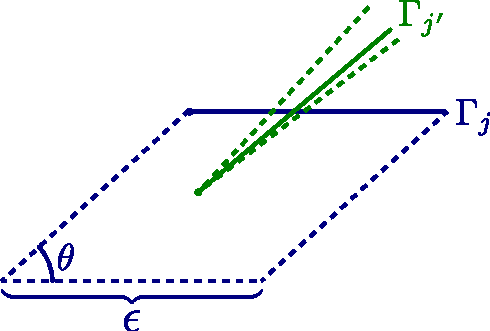
\includegraphics[scale=0.8]{Figures/Rhombus.pdf} 
\caption{$\Gamma_j$ and $\Gamma_{j'}$ intersect in an angle close to $\theta$.}\label{fig:Rhombus}
\end{figure}


Consider, in particular, the number of self-intersections of $\gamma[0,T)$. For $\theta \in [0, \pi]$ and for any pair of indices $j,j'$, the event $F_{j,j'}(\theta; d\theta)$ that the projections to $S$ of the segments $\Gamma_{j}$ and $\Gamma_{j'}$ cross at angle between $\theta- d\theta$ and $\theta+ d\theta$ is, up to an error of size $O(d\theta)$, the same as the event that (i) the point $\gamma(j' \varepsilon) $ lies in a rhombus on $S$ whose sides meet at angle $\theta$ and whose ``top'' side is the projection to $S$ of $\Gamma_{j}$, and (ii) the tangent angle of $\tilde{\gamma}(j' \varepsilon)$ differs from that of $\tilde{j \varepsilon}$ by $\theta \pm d \theta$ (Figure~\ref{fig:Rhombus}). (Similarly, for $\Gamma_{j}$ and $\Gamma_{j'}$ to cross at angle $\pi+ (\theta \pm d\theta)$ the ``bottom'' side of the rhombus should be the projection of $\Gamma_{j}$.) Since $\Gamma_{j}$ and $\Gamma_{j'}$ are approximately independent, the probability of this event is (approximately) the relative area of this rhombus times $2 d\theta$ divided by $2\pi$. Summing over $\theta$ and taking $d\theta \rightarrow 0$ now shows that the probability of intersection is about
\[
\frac{2 \varepsilon^{2} \int_{0}^{\pi} \sin \theta \, d\theta}{2\pi\area(S)}= \frac{2 \varepsilon ^{2}\kappa}{\pi}
\]
where $\kappa=(1/ \area(S))$. This fails, of course, if $|j-j'|$ is small, but for most pairs $j,j'$ the difference will be large. Consequently, by the law of large numbers, the number of self-intersections of the segment $\gamma[0,T]$, when divided by $T^{2}$, should satisfy
\[
\frac{1}{T^{2}} \sum_{j=1}^{N}\sum_{j'=j+1}^{N}\mathbf{1} \xset{\Gamma_{j'} \text{ crosses } \Gamma_{j}} \approx
\frac{\kappa}{\pi}.
\]

Amplification of this argument ``explains'' the local convergence of the induced tessellation to the Poisson line process. Consider, for instance, the number of distinct geodesic arcs that cross the disk $D(x, \alpha/T)$, for some fixed point $x \in S$: we will argue that this should have approximately a Poisson distribution. Choose $\varepsilon$ small, and let $T=N \varepsilon$ be an integer multiple of $\varepsilon $ large enough that $1/T \ll \varepsilon$. For each $j\leq N$, the probability that (the projection of) $\Gamma_{j}$ crosses the disk $D(x, \alpha T^{-1})$ is, for small $\varepsilon$, about $C\varepsilon \alpha /T=C \alpha /N$ for a suitable geometric constant $C>0$. (This follows by a simple geometric argument similar to that given above for self-intersections.) Thus, if the random segments $\Gamma_{j}$ were actually independent, the number that would cross the disk $D(x, \alpha /T)$ would be the sum of $N$ independent Bernoulli random variables each with mean $C \alpha /N$. For $N$ large, the distribution of this count would therefore converge to Poisson with mean $C \alpha$ (cf. Proposition~\ref{proposition:lsn} below).

The sticky point, of course, is that the random segments $\Gamma_{j}$ are not independent. What is worse, the events of interest (for instance, the event that $\Gamma_{j}$ crosses the disk $D(x,\alpha T^{-1})$) are events whose probabilities become small as $N$ becomes large; thus, the mixing property of the geodesic flow does not by itself imply that
\[
\frac{P (\xset {\Gamma_{j} \text{ crosses } D(x,\alpha T^{-1})}\cap \xset {\Gamma_{j'} \text{ crosses } D(x,\alpha T^{-1})})}{P \xset {\Gamma_{j} \text{ crosses } D(x,\alpha T^{-1})}P \xset {\Gamma_{j'} \text { crosses }D(x,\alpha T^{-1})}} \approx 1
\]
even for $|j-j'| $ large. The rigorous arguments to be given below are largely designed to circumvent the failure of mixing at this level by exploiting the Gibbsean structure of the Liouville measure.

Mixing problems in which the events of interest have probabilities tending to zero are known as ``shrinking target'' problems. Such problems occur naturally in hyperbolic dynamics: see, for instance, \cite{Sullivan}, where the ``target'' is one of the cusps of a non-compact hyperbolic surface of finite area, or Kleinbock--Margulis~\cite{KM}, who consider related problems for diagonal flows on finite-volume homogeneous spaces. For shrinking target problems where the targets lie in the compact part of the space, see Dolgopyat~\cite{Dolgopyat2}, and Maucourant~\cite{Maucourant}. Unfortunately none of these results is easily adapted to the problems we consider here.



\subsection{Global Statistics}\label{ssec:global}

Theorems~\ref{theorem:random-local}--\ref{theorem:random-local-pairs} describe the ``local'' structure of the random tessellation $\mathcal{T}_{T}$ of the surface $S$ induced by a long segment$\gamma[0,T]$ of a random geodesic. The tessellation $\mathcal{T}_{T}$ will consist of geodesic polygons, typically of diameter of order $T^{-1}$, since the $O (T^{2})$ self-intersections will subdivide the length $T$ geodesic segment into sub-segments of length $O (T^{-1})$. Thus, it is natural to look at the statistics of the scaled tessellation $T\mathcal{T}_{T}$, which we view as consisting of a random number of triangles, quadrilaterals, etc., each with its own set of side-lengths and interior angles.

The empirical frequencies of triangles, quadrilaterals, etc. and the empirical distribution of side-length and interior-angle sets in a Poisson line process of intensity $\kappa$ on the ball $B (0; \alpha)$ of radius $\alpha$ converge as $\alpha \rightarrow \infty$. (These results are evidently due to R. E. Miles~\cite{miles:pnas1,miles:pnas2}; proofs are given in Section~\ref{sec:preliminaries} below.) Theorem~\ref{theorem:random-local} asserts that when $L$ is large, then for any point $x\in S$ the statistics of the polygonal partition in $B (x;\alpha^{-1}L)$ induced by a random geodesic segment of length $L$ should approach those of a Poisson line process. From this observation we will deduce the following assertion regarding \emph{global} statistics.



\begin{theo}\label{theorem:global-stats}
Let $\mathcal{T}_{T}$ be the tessellation of $S$ induced by a random geodesic of length $T$. Then with probability approaching $1$ as $T \rightarrow \infty$, the empirical frequencies of triangles, quadrilaterals, etc. and the empirical distribution of side-length and interior-angle sets in $\mathcal{T}_{T}$ approach the corresponding theoretical frequencies for a Poisson line process.
\end{theo}


For example, for each $v \in T^1(S)$, let $\mathcal T_T(v)$ be the tessellation induced by the length $T$ arc with initial direction~$v$. Let $f_3$ be the function that returns the frequency of triangles in a tessellation. Suppose the expected value of $f_3$ is $\tau_3$ for a Poisson line process. Then we show that for any $\epsilon > 0$,
\[
\lim_{T \to \infty} \mu_L \left\{v \in T^1(S) \,:\, |f_3(\mathcal T_T(v)) - \tau_3| > \epsilon\right\} = 0
\]
where $\mu_L$ is the Liouville measure on $T^1(S)$.

\subsection*{Plan of the paper.}
The proofs of Theorems~\ref{theorem:random-local}--\ref{theorem:random-local-pairs} will occupy most of the paper. The strategy will be to reduce the problem to a corresponding counting problem in symbolic dynamics. Preliminaries on Poisson line processes will be collected in Section~\ref{sec:preliminaries}, and preliminaries on symbolic dynamics for the geodesic flow in Section~\ref{sec:symbolicDynamics}. Section~\ref{sec:heuristics} will be devoted to heuristics and a reformulation of the problem; the proofs of Theorems~\ref{theorem:random-local}--\ref{theorem:random-local-pairs} will then be carried out in Sections~\ref{sec:no-prefixes}--\ref{sec:final-step}. Theorem~\ref{theorem:global-stats} will be proved in Section~\ref{sec:global-stats}. Finally, in Section~\ref{sec:ext}, we give a short list of conjectures, questions, and possible extensions of our main results.


\section{Preliminaries: Poisson line processes} \label{sec:preliminaries}
The Poisson line process and its generalizations have a voluminous literature, with notable early contributions by Miles~\cite{miles:pnas1,miles:pnas2}. See~\cite{kendall-et-al} for an extended discussion and further pointers to the literature. In this section we will record some basic facts about these processes. These are mostly known -- some of them are stated as theorems in~\cite{miles:pnas1} without proofs -- but proofs are not easy to track down, so we shall provide proof sketches in Appendix~\ref{sec:appendix}.



\subsection{Statistics of a Poisson line process}\label{ssec:plp}

\begin{lemm}\label{lemma:translation-invariance}
A Poisson line process of constant intensity $\kappa$ is rotationally and translationally invariant, that is, if $A$ is any orientation preserving isometry of $\zz{R}^{2}$ then the configuration $\{AL_{n} \}_{n\,\in\,\zz{Z}}$ has the same joint distribution as the configuration $\{L_{n} \}_{n\,\in\,\zz{Z}}$.
\end{lemm}

\begin{rema}\label{remark:ti}
This result is stated without proof in~\cite{miles:pnas1}. A proof of the corresponding fact for the intensity measure can be found in~\cite{santalo}, and another in~\cite[Chapter~8]{kendall-et-al}. A short, elementary proof is given in Appendix~\ref{sec:appendix}. The following Corollary~\ref{corollary:line-intensity}, which is stated without proof as~\cite[Theorem~2]{miles:pnas1}, follows easily from isometry-invariance.
\end{rema}

\begin{coro}\label{corollary:line-intensity}
Let $\mathcal{L}$ be a Poisson line process of intensity $\kappa>0$. For any fixed line $\ell$ in $\mathbb{R}^{2}$, the point process of intersections of $\ell$ with lines in $\mathcal{L}$ is a Poisson point process of intensity $2\kappa /\pi$.
\end{coro}


\begin{lemm}\label{lemma:local-sparsity}
Let $\mathcal{L}$ be a Poisson line process of intensity $\kappa >0$, and for each point $x\in\mathbb{R}^{2}$ and each real $r>0$ let $N(B(x;r))$ be the number of lines in $\mathcal{L}$ that intersect the ball $B(x;r)$ of radius $r$ centered at $x$. Then the random variable $N(B(x;r))$ has the Poisson distribution with mean $2\kappa r$. Consequently, with probability one, for any compact set $K\subseteq \zz{R}^{2}$ the set of lines $L_{n}$ in $\mathcal{L}$ that intersect $K$ is finite.
\end{lemm}

\begin{proof}
Without loss of generality, take $K=B(0;R)$ to be the closed ball of radius $R$ centered at the origin. Then the line $L_{n}$ intersects $K$ if and only if $|R_{n}|\leq R$. Since a Poisson point process on $\zz{R}$ of constant intensity has at most finitely many points in any finite interval, the result follows.
\end{proof}



The next result {characterizes} the Poisson line process (see also Proposition~\ref{proposition:sufficientCondition} below). Fix a bounded, {convex} region $D\subset \mathbb{R}^{2}$ with $C^{\infty}$ boundary $\Gamma =\partial D$, and let $A,B$ be non-intersecting closed arcs on $\Gamma$. For any line process $\mathcal{L}$, let
\begin{equation}\label{eq:crossingCounts}
N_{\{A,\,B\}}= \# \,\left\{\text{lines that cross both}\; A \;\text{and}\;B\right\}.
\end{equation}
For any angle $\theta \in [-\pi /2,\pi /2]$, the set of lines that intersect both $A$ and $B$ and meet the $x-$axis at angle $\theta +\pi /2$ constitute an infinite strip that intersects the line $\{re^{i\theta} \}_{r\,\in \,\zz{R}}$ in an interval; see Figure~\ref{fig:Strip at angle theta} below. Let $\psi (\theta)=\psi_{A,\,B} (\theta)$ be the length of this interval, and define
\begin{equation}\label{eq:beta}
\beta_{A,\,B}=\frac{1}{\pi} \int_{-\pi /2}^{\pi /2}\psi (\theta)\,d\theta.
\end{equation}


\begin{figure}[h!]
\centering
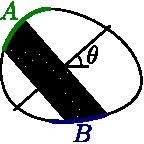
\includegraphics{Figures/ConnectBoundaryArcs-eps-converted-to.pdf} 
%\includegraphics[scale=1]{ConnectBoundaryArcs-eps-converted-to.pdf}
\caption{Lines that cross $A$ and $B$ at angle $\theta$.}\label{fig:Strip at angle theta}
\end{figure}

\goodbreak
\begin{prop}\label{proposition:characterization}
A line process $\mathcal{L}$ in $D$ is a Poisson line process of rate $\kappa >0$ if and only if
\begin{enumerate}\romanenumi
\item \label{list2.5.1}for any two non-intersecting arcs $A,B \subset \Gamma$, the random variable $N_{\xset {A,\,B}}$ has the Poisson distribution with mean $\kappa \beta_{A,B}$, and
\item \label{list2.5.2}for any finite collection $\{A_{i},\,B_{i} \}_{i\,\leq\,m}$ of pairwise disjoint boundary arcs, the random variables $N_{\{A_{i},\,B_{i}\}}$ are mutually independent.
\end{enumerate}
\end{prop}

See Appendix~\ref{sec:appendix} for the proof of the forward implication, along with that of the following corollary. The converse implication in Proposition~\ref{proposition:characterization} will follow from Proposition~\ref{proposition:sufficientCondition} in Section~\ref{ssec:poissonApprox} below.


\begin{coro}\label{corollary:ppIntensity}
Let $D\subset \zz{R}^{2}$ be a compact, convex region, and let $\mathcal{L}$ be a Poisson line process with intensity $\kappa$. The number $V(D)$ of intersection points (vertices) of $\mathcal{L}$ in $D$ has expectation
\[
EV (D)=\kappa^{2} |D|/\pi
\]
where $|D|$ is the Lebesgue measure of $D$.
\end{coro}



\subsection{Ergodic theorem for Poisson line processes}\label{ssec:erg-theorem-plp}

The configuration space $\mathcal{C}$ in which a Poisson line process takes values is the set of all countable, locally finite collections of lines in $\zz{R}^{2}$. This space has a natural metric topology, specifically, the weak topology generated by the Hausdorff topologies on the restrictions to balls in $\zz{R}^{2}$. Moreover, $\mathcal{C}$ admits an action (by translations) of $\zz{R}^{2}$. Denote by $\nu_{\kappa}$ the distribution of the Poisson line process with intensity $\kappa$. By Lemma~\ref{lemma:translation-invariance}, the measure $\nu_{\kappa}$ is translation-invariant.

\begin{prop}\label{proposition:ergodicity-plp}
The probability measure $\nu_{\kappa}$ is mixing (and therefore ergodic) with respect to the translational action of $\zz{R}^{2}$ on $\mathcal{C}$.
\end{prop}

\begin{rema}\label{remark:kendall}
Ergodicity of the measure $\nu_{\kappa}$ is asserted in Miles' papers~\cite{miles:pnas1,miles:pnas2}, and proved in his unpublished Ph.~D. dissertation. We have been unable to locate a proof in the published literature, so we have provided one in the Appendix.
\end{rema}

\begin{coro}\label{corollary:poly-freqs}
Let $\Phi _{n,\,k}$ be the fraction of $k-$gons, $F_{n}$ (for ``faces'') the total number of polygons, and $V_{n}$ (for ``vertices'') the number of intersection points in the tessellation of the square $[-n,n]^{2}$ induced by a Poisson line process $\mathcal{L}$ of intensity $\kappa$. There exist constants $\phi _{k}>0$ such that with probability $1$,
\begin{align}\label{eq:poly-freqs}
&\lim_{n \rightarrow \infty} F_{n}/ (2n)^{2}=\kappa^{2} /\pi,\\\label{eq:vertex-freqs}
&\lim_{n \rightarrow \infty} V_{n}/ (2n)^{2}=\kappa^{2}/\pi, \quad \text{and}\\\label{eq:kgonFracs}
&\lim_{n \rightarrow \infty} \Phi _{n,\,k}=\phi _{k}.
\end{align}
\end{coro}

Integral formulas for the quantities $\phi_k$ are given in~\cite{Calka}.

The ergodic theorem can also be used to prove that a variety of other statistical properties stabilize in large squares. Consider, for example, the number $N_{n} (A,B,C)$ of triangles contained in $[-n,n]^{2}$ whose side lengths $\alpha,\beta,\gamma$ lie in the intervals $A,B,C$; then as $n
\rightarrow \infty$,
\[
N_{n} (A,B,C)/ (2n)^{2} \longrightarrow E \mathbf{1}_{G (A,\,B,\,C)} (\mathcal{L})
\]
where $G (A,B,C)$ is the event that the polygon containing the origin is a triangle with side lengths in $A,B,C$.


\subsection{Weak convergence to a Poisson line process}\label{ssec:poissonApprox}

For any unordered pair $\{A,B \}$ of non-overlapping boundary arcs of the disk $B (0,\alpha)$, let $L_{\{A,\,B \}}$ be the set of lines in $\zz{R}^{2}$ that intersect both $A$ and $B$. This set can be identified with the set of point pairs $\{x,y \}$ where $x\in A$ and $y\in B$. This allows us to view any random collection of unordered point pairs $\{x,y \}$ as a \emph{line process} in $B (0,\alpha)$, even when the collection consists of endpoints of arcs across $B (0,\alpha)$ that are not line segments (in particular, when they are pullbacks of geodesic arcs to the tangent space). For any line process $\mathcal{L}$ in $B (0,\alpha)$ let $N_{\{A,\,B \}}$ be the cardinality of $\mathcal{L}\cap L_{\{A,\,B \}}$ (cf. equation~\eqref{eq:crossingCounts}).

\begin{prop}\label{proposition:sufficientCondition}
Let $\mathcal{L}_{n}$ be a sequence of line processes in $B (0;\alpha)$, and let $\mu_{n}$ be the distribution of $\mathcal{L}_{n}$ (i.e., the probability measure on $\mathcal{X}$ induced by $\mathcal{L}_{n}$). In order that $\mu_{n}\rightarrow \mu$ weakly, where $\mu$ is the law of a rate$-\kappa$ Poisson line process, it suffices that the following condition holds. For any finite collection $\{\{ A_{i},\,B_{i}\} \}_{i\,\leq\,m}$ of unordered pairs of non-overlapping boundary arcs of $B(0;\alpha)$ such that the sets $L_{\{A_{i},\,B_{i} \}}$ are pairwise disjoint, the joint distribution of the counts $N_{\{ A_{i},\,B_{i}\}}$ under $\mu_{n}$ converges to the joint distribution under $\mu$, that is, for any choice of nonnegative integers $k_{i}$,
\begin{equation}\label{eq:suff-weak-convergence}
\lim_{n \rightarrow \infty} \mu_{n}\left\{N_{\{A_{i},\,B_{i} \}}=k_{i} \; \forall \,i\leq m\right\} =\prod_{i=1}^{m}
\frac{(\kappa \beta_{A_{i},\,B_{i}})^{k_{i}}}{k_{i}!} e^{-\kappa \beta_{A_{i},\,B_{i}}}.
\end{equation}
\end{prop}



\begin{proof}
[Proof Sketch] Recall that the configuration space $\mathcal{X}$ is the disjoint union of the sets $\mathcal{X}_{k}$, where $\mathcal{X}_{k}$ is the set of all finite sets $F=\{\{x_{i},y_{i} \} \}_{1\,\leq\,i\,\leq\, k}$ consisting of $k$ unordered pairs of points on $\partial B (0,\alpha)$. Since each set $\mathcal{X}_{k}$ is both open and closed in $\mathcal{X}$, to prove weak convergence $\mu_{n}\rightarrow \mu$ it suffices to establish the convergence~\eqref{eq:weak-conv-definition} for every continuous function $f$ supported by just one of the sets $\mathcal{X}_{k}$.

For each $k$, the space $\mathcal{X}_{k}$ is a quotient of $(\partial B (0,\alpha)^{2})^{k}$ with the usual topology, and so every continuous function $f:\mathcal{X}_{k}\rightarrow \zz{R}$ can be uniformly approximated by ``step functions'', that is, functions $g$ of configurations $F=\{\{x_{i},\,y_{i} \} \}_{1\,\leq\,i\,\leq\,k}$ that depend only on the counts $N_{A_{i},\,B_{i}}$ for arcs $A_{i},B_{i}$ in some partition of $\partial B (0,\alpha)$. If~\eqref{eq:suff-weak-convergence} holds, then it follows by linearity of expectations that for any such step function $g$,
\[
\lim_{n \rightarrow \infty} \int g\,d\mu_{n}=\int g\,d\mu,
\]
and hence~\eqref{eq:weak-conv-definition} follows.
\end{proof}



\subsection{The ``law of small numbers''}\label{ssec:lsn}
A elementary theorem of discrete probability theory states that for large $n$, the Binomial$- (n,\kappa /n)$ distribution is closely approximated by the Poisson distribution with mean $\kappa$. The following is a generalization that we will find useful.

\begin{prop}\label{proposition:lsn}
Let $X_{1},X_{2},\,\dotsc,\,X_{n}$ be independent Bernoulli random variables with success parameters $EX_{i}=p_{i}$. Let $\alpha =\max_{i}p_{i}$ and $\kappa =\sum_{i}p_{i}$. Then there is a constant $C<\infty$ not depending on $p_{1},p_{2},\,\dotsc,\,p_{n}$ such that
\[
\sum_{k=0}^{\infty} \left\lvert P\left\{\sum_{i}X_{i}=k
\right\}-\frac{\kappa^{k}}{k!}e^{-\kappa}\right\rvert \leq C\alpha.
\]
\end{prop}

Note that for all $k > n$, the probability $P\left\{\sum_{i}X_{i}=k \right\}$ is zero, but the elements of the sum are not.

See~\cite{lecam} for a proof. The important feature of the proposition for us is not the explicit bound, but the fact that the closeness of the approximation depends only on $\max p_{i}$.

A similar result holds for multinomial variables.

\begin{prop}\label{proposition:mult-lsn}
Let $X_{1},X_{2},\dotsc,X_{n}$ be independent random variables each taking values in the finite set $\{0,1,2,\dotsc,K \}=\{0\} \cup [K]$, and for each pair $i,j$ set $p_{i,\,j}=P\{X_{i}=j \}$. Let $\alpha =\max_{j\,\geq\,1}\max_{i}p_{i,\,j}$ and $\kappa_{j}=\sum_{i}p_{i,\,j}$, and for each $j$define
\[
T_{j}=\sum_{i=1}^{n}\mathbf{1}\{X_{i}=j \}.
\]
Then there is a function $C_{K} (\alpha)$ satisfying $\lim_{\alpha \downarrow 0}C (\alpha)=0$ such that
\[
\sum_{m_{1}=0}^{\infty}\,\sum_{m_{2}=0}^{\infty}\dotsb
\sum_{m_{K}=0}^{\infty}
\left\lvert P\left\{T_{j}=m_{j} \;\forall \, j\in [K]\right\} -\prod_{j=1}^{K}\kappa_{j}^{m_{j}}e^{-\kappa_{j}}/m_{j}! \right\rvert \leq C (\alpha).
\]
\end{prop}



\section{Preliminaries: Symbolic Dynamics}\label{sec:symbolicDynamics}

\subsection{Shifts and suspension flows}\label{ssec:suspFlows}

The geodesic flow on the unit tangent bundle $T^1S$ of a compact, negatively curved surface $S$ has a concrete representation as a suspension flow over a shift of finite type. In describing this representation, we shall follow (for the most part) the terminology and notation of~\cite{bowen:book,lalley:duke,series:symbDynFlows}. Let $\mathcal{A}$ be a finite alphabet and $\mathcal{F}$ a finite set of finite words on the alphabet $\mathcal{A}$, and define $\Sigma =\Sigma_{\mathcal{F}}$ to be the set of doubly infinite sequences $\omega = (\omega_{n})_{n\,\in\, \zz{Z}}$ such that no element of $\mathcal{F}$ occurs as a subword of $\omega$. The sequence space $\Sigma $ is given the metric $d (\omega,y)=\exp \{-n (\omega,y) \}$ where $n (\omega,y)$ is the minimum nonnegative integer $n$ such that $\omega_{j}\not =y_{j}$ for $j= n$ or $j=-n$. For each nonnegative integer $m$ and each $\omega \in \Sigma$, define the \emph{cylinder set} $\Sigma_{m}(\omega) $ to be the set of all $\omega'\in\Sigma$ that agree with $\omega$ in all coordinates $j$ such that $|j| \leq m$; equivalently,
\begin{equation}\label{eq:cylinder}
\Sigma_{m}(\omega)= \xset {\omega' \in \Sigma \,:\, d(\omega,\omega')< e^{-m}}.
\end{equation}
The forward shift $\sigma :\Sigma \rightarrow \Sigma$ is known as a (two-sided) \emph{shift of finite type}.\footnote{Bowen~\cite{bowen:book} requires that the elements of the set $\mathcal{F}$ all be of length 2. However, any shift of finite type can be ``recoded'' to give a shift of finite type obeying Bowen's convention, by replacing the original alphabet $\mathcal{A}$ by $\mathcal{A}^{m}$, where $m$ is the length of the longest word in $\mathcal{F}$, and then replacing each sequence $\omega $ by the sequence $\bar{\omega}$ whose entries are the successive length-$m$ subwords of $\omega$. In Series'~\cite{series:symbDynFlows} symbolic dynamics for the geodesic flow on a closed hyperbolic surface, the alphabet $\mathcal{A}$ is a set of natural generators for the fundamental group $\pi_{1} (S)$ of the surface $S$, and the forbidden subwords $\mathcal{F}$ are gotten from the relators of $\pi_{1} (S)$.}



For any continuous function $F:\Sigma \rightarrow (0,\infty)$ on $\Sigma$, define the \emph{suspension space} $\Sigma_{F}$~by
\[
\Sigma_{F} :=\{(\omega,t)\,:\, \omega\in \Sigma \;\; \text{and} \; 0\leq t\leq F (\omega)\},
\]
with points $(\omega,F (\omega))$ and $(\sigma \omega,0)$ identified. The metric $d$ on the sequence space $\Sigma$ induces a metric $d_{\textsc{Taxi}}$ on $\Sigma_{F}$, the ``taxicab'' metric. (Roughly, the distance between any two points $(\omega, t)$ and $(\omega',t')$ in $\Sigma_{F}$ is the length of the shortest ``path'' between them consisting of alternating ``horizontal'' and ``vertical'' segments. See~\cite{bowen-walters} for the formal definition.) The \emph{suspension flow} with height function $F$ is the flow $\phi_{t}$ on $\Sigma_{F}$ whose orbits proceed up vertical fibers
\[
\mathcal{F}_{\omega}:=\{(\omega,s)\,:\,0\leq s\leq F (\omega) \}
\]
at speed $1$, and upon reaching the ceiling at $(\omega,F (\omega))$ jump instantaneously to $(\sigma \omega,0)$. If the height function $F: \Sigma \rightarrow \mathbb{R}$ is H\"older continuous with respect to the metric $d$, then the suspension flow $\phi_{t}$ is H\"older continuous with respect to the metric $d_{\textsc{Taxi}}$: in particular, there exists $\alpha>0$ such that
\begin{equation}\label{eq:suspFlowHolder}
d_{\textsc{Taxi}}(\phi_{t}(\omega,0), \phi_{t}(\omega',0))\leq e^{\alpha |t|}d(\omega,\omega') \quad \text{for all} \quad
\omega,\omega'\in\Sigma \; \text{and} \; t \in \mathbb{R}.
\end{equation}



There is a bijective correspondence between invariant probability measures $\mu^{*}$ for the flow $\phi_{t}$ and shift-invariant measures $\mu$ on $\Sigma$. This correspondence can be specified as follows: for any continuous function $g:\Sigma_{F} \rightarrow \zz{R}$,
\begin{equation}\label{eq:measure-transfer}
\int g\, d\mu^{*}=\int_{\Sigma}\int_{0}^{F (\omega)} g (\omega,s) \,ds\,d\mu (\omega) /\int_{\Sigma}F\,d\mu.
\end{equation}
If $\mu$ is ergodic for the shift $(\Sigma,\sigma)$ then $\mu^{*}$ is ergodic for the flow $(\Sigma_{F},\phi_{t})$. By Birkhoff's theorem, for any ergodic probability measure $\mu$ on $\Sigma$,
\begin{equation}\label{eq:birkhoff-F}
\lim_{n \rightarrow \infty}n^{-1}\sum_{j=0}^{n-1}F\circ\sigma^{j} =\int_{\Sigma}F\,d\mu \quad \text{almost surely};
\end{equation}
thus, under $\mu^{*}$, almost every orbit makes roughly $T/\int F\,d\mu$ visits to the base $\Sigma \times \{0 \}$ by time $T$, when $T$ is large.



\subsection{Symbolic dynamics for the geodesic flow}\label{ssec:symbDynGF}

The following Proposition~\ref{proposition:boundaryCorrespondence} is a special case of the main result of~\cite{ratner:markov} (see also~\cite{bowen:symbDyn}), as the geodesic flow on a compact, negatively curved surface is an Anosov flow.

\begin{prop}\label{proposition:boundaryCorrespondence}
For any compact, negatively curved surface $(S, \varrho)$ with $C^{\infty}$ Riemannian metric $\varrho$, there exist a topologically mixing shift $(\Sigma,\sigma)$ of finite type, a suspension flow $(\Sigma_{F},\phi_{t})$ over the shift with H\"older continuous height function $F$, and a surjective, H\"older-continuous mapping $\pi:\Sigma_{F} \rightarrow T^1S$ such that $\pi$ is a semi-conjugacy with the geodesic flow $\gamma_{t}$ on $T^1S$, i.e.,
\begin{equation}\label{eq:semi-conjugacy}
\pi \circ \phi_{t}=\gamma_{t} \circ \pi \quad \text{for all}\;\;t\in \zz{R}.
\end{equation}
\end{prop}


In the special case where $\varrho$ is a hyperbolic (constant curvature) Riemannian metric, a much more explicit symbolic dynamics was constructed by Series: see especially~\cite[Theorem~3.1]{series:symbDynFlows} and also~\cite{bowen-series}. In this symbolic dynamics, the sequence space $\Sigma$ is mapped to a subset of $\partial \mathbb{D}\times \partial \mathbb{D}$, where $\partial \mathbb{D}$ is the ideal boundary of the Poincaré disk, in such a way that every vertical fiber $\mathcal{F}_{\omega}$ of the suspension flow is mapped to a segment of the hyperbolic geodesic in $\mathbb{D}$ whose endpoints are gotten from the boundary correspondence. Series' symbolic dynamics can be extended to the variable curvature case using the \emph{Conformal Equivalence Theorem} (\cite[Theorem~V.1.3]{schoen-yau}) and the structural stability theorem for Anosov flows. This more explicit symbolic dynamics will not be needed in the analysis below. However, we will need the following fact (see~\cite[Chapter~7]{paulin-pollicott-schapira}).

\begin{prop}\label{proposition:LiouvilleGibbs}
Under the hypotheses of Proposition~\ref{proposition:boundaryCorrespondence}, the pullback $\lambda^{*}:=\mu_{L}\circ \pi^{-1}$ of the normalized Liouville measure $\mu_{L}$ on $T^{1}S$ is Gibbs, that is, it corresponds to a Gibbs state $\lambda$ for the shift via the identity~\eqref{eq:measure-transfer}.
\end{prop}


\subsection{Regenerative representation of Gibbs states}\label{ssec:regeneration}

When the underlying shift $(\Sigma,\sigma)$ is topologically mixing, Gibbs states with H\"older continuous potentials enjoy strong exponential mixing properties (e.g.,~\cite[the ``exponential cluster property''~1.26 in Chapter~1]{bowen:book}). We shall make use of an even stronger property, the \emph{regenerative representation} of a Gibbs state established in~\cite{lalley:regeneration}.\footnote{The article~\cite{lalley:regeneration} proves the regenerative representation only for Gibbs states defined on a full shift, but the arguments are easily modified for topologically mixing shifts of finite type. See also~\cite{comets-et-al} for a somewhat different approach.} This representation is most usefully described in terms of the stationary process governed by the Gibbs state. Let $\mu$ be a Gibbs state with H\"older continuous potential function $f:\Sigma \rightarrow \mathbb{R}$, where $\sigma :\Sigma \rightarrow \Sigma$ is a topologically mixing shift of finite type, and let $X_{n}:\Sigma \rightarrow \mathcal{A}$ be the coordinate projections on $\Sigma$, for $n\in \zz{Z}$. The sequence $(X_{n})_{n\,\in\,\zz{Z}}$, viewed as a stochastic process on the probability space $(\Sigma,\mu)$, is a stationary process that we will henceforth call a \emph{Gibbs process}.

The regenerative representation relates the class of Gibbs processes to another class of stationary processes, called \emph{list processes} (the term used by~\cite{lalley:regeneration}). A list process is a stationary, positive-recurrent Markov chain $(Z_{n})_{n\,\in\,\zz{Z}}$ with state space $\cup_{k\,\geq\,1}\mathcal{A}^{k}$ and stationary distribution $\nu$ that obeys the following transition rules: first,
\begin{equation}\label{eq:list-1}
P \big(Z_{n+1}= (\omega_{1},\omega_{2},\dotsc,\omega_{m})\,\big|\, Z_{n}= (\omega '_{1},\omega '_{2},\dotsc, \omega '_{k})\big)=0
\end{equation}
unless either $m=1$ or $m=k+1$ and $\omega_{i}=\omega '_{i}$ for each $1\leq i\leq k$; and second, for every letter $\omega_{1}$ and every word $\omega '_{1}\omega '_{2}\dotsb \omega '_{m}$,
\begin{equation}\label{eq:list-2}
P \big(Z_{n+1}=\omega_{1}\,\big|\, Z_{n+1}\in \mathcal{A}^{1} \;\text{and}\; Z_{n}= (\omega '_{1},\omega '_{2},\dotsb,\omega '_{m})\big) =\nu ((\omega_{1}))/\nu (\mathcal{A}^{1}).
\end{equation}
Thus, the process $(Z_{n})_{n\,\in\,\zz{Z}}$ evolves by either adding one letter to the end of the list or erasing the entire list and beginning from scratch. Furthermore, by~\eqref{eq:list-2}, at any time when the list is erased, the new 1-letter word chosen to begin the next list is independent of the past history of the entire process.

For any list process define the \emph{regeneration times} $0=\tau_{0}<\tau_{1}<\tau_{2}<\dotsb$ by
\begin{align*}
\tau_{1}&=\min \left\{n\geq 1\,:\, Z_{n}\in \mathcal{A}^{1}\right\};\\
\tau_{m+1}&=\min \left\{n\geq 1+\tau_{m}\,:\, Z_{n}\in \mathcal{A}^{1}\right\}.
\end{align*}
By condition~\eqref{eq:list-2}, the random variables $\tau_{m+1}-\tau_{m}$ are independent, and for $m\geq 1$ are identically distributed, as are the \emph{excursions}
\[
\left(Z_{\tau_{m}+1},Z_{\tau_{m}+2},\dotsc,Z_{\tau_{m+1}}\right).
\]
Denote by $\pi :\cup_{k\,\geq\,1}\mathcal{A}^{k} \rightarrow \mathcal{A}$ the projection onto the \emph{last} letter.

\begin{prop}\label{proposition:regeneration}
If $(X_{n})_{n\,\in\,\zz{Z}}$ is a Gibbs process then there is a list process $(Z_{n})_{n\,\in\,\zz{Z}}$ such that the projected process $(\pi (Z_{n}))_{n\,\in\,\zz{Z}}$ has the same joint distribution as the Gibbs process $(X_{n})_{n\,\in\,\zz{Z}}$. Thus, the random sequence obtained by concatenating the successive excursions $W_{m}:=Z_{\tau_{m}}$, i.e.,
\[
W_{1}\cdot W_{2}\cdot W_{3}\cdot\dotsb,
\]
has the same distribution as the sequence $\{X_{n} \}_{n\, \geq\,0}$. Moreover, the list process can be chosen in such a way that the excursion lengths $\tau_{m+1}-\tau_{m}$ satisfy
\begin{equation}\label{eq:exp-regeneration}
P (\tau_{m+1}-\tau_{m}\geq n)\leq C\alpha^{n}
\end{equation}
for some $0<\alpha <1$ and $C<\infty$ not depending on either $m$ or $n$.
\end{prop}

See~\cite[Theorem~1]{lalley:regeneration}, or~\cite[Theorem~4.1.]{comets-et-al}, (The article~\cite{lalley:regeneration} uses the (older) term \emph{chain with complete connections} for a Gibbs process, and a different (but equivalent) definition than that given in~\cite{bowen:book}. Moreover,\cite{lalley:regeneration} considers only the case where the underlying shift is the full shift on the symbol set $\mathcal{A}$, although the proof extends routinely to the general case. See~\cite{li-naud-pan} for details.)



\section{Theorem~\ref{theorem:random-local} Proof: Strategy}\label{sec:heuristics}

We shall use the symbolic dynamics outlined in Section~\ref{ssec:symbDynGF} to translate the weak convergence problem to a problem involving the Gibbs state $\lambda$ corresponding to the pullback $\lambda^{*}$ of Liouville measure to the suspension space $\Sigma_{F}$. Recall (cf. Proposition~\ref{proposition:boundaryCorrespondence}) that the projection $\pi:\Sigma_{F}\rightarrow T^{1}S$ provides a semi-conjugacy~\eqref{eq:semi-conjugacy} between the suspension flow $\phi_{t}$ and the geodesic flow $\gamma_{t}$; thus, each segment of the suspension flow projects (via the mapping $p\circ\pi$, where $p:T^{1}S\rightarrow S$ is the natural projection) to a geodesic segment of the same length, and in particular, each fiber $\mathcal{F}_{\omega}$ of the suspension space $\Sigma_{F}$ projects to a geodesic segment of length $F(\omega)$.


By Birkhoff's ergodic theorem (cf. equation~\eqref{eq:birkhoff-F}), for $\lambda-$almost every $\omega \in
\Sigma$, the number of returns to the base $\Sigma \times \xset {0}$ made by the suspension flow by time $T$, divided by $T$, converges to $1/E_{\lambda}F $. We will show (cf. Proposition~\ref{proposition:no-quick-entries} in Section~\ref{sec:no-prefixes} below) that for any $\alpha>0$, the probability that a random geodesic enters the disk $D(x,\alpha T^{-1})$ between times $(1- \varepsilon)T$ and $(1+ \varepsilon)T$ is bounded by $C\varepsilon$ for some $C=C(\alpha)<\infty$ not depending on $T$. Consequently, with $\lambda-$probability approaching $1$ as $T\rightarrow\infty$, the intersection of the random geodesic segment $p \circ \pi (\phi_{[0,\,T]}(\omega))$ with $D(x, \alpha T^{-1})$ is identical to the intersection of $D(x, \alpha T^{-1})$ with the geodesic segment
\begin{equation}\label{eq:n}
p\circ\pi(\cup _{i=0}^{n(T)-1}\mathcal{F}_{\sigma^{i}\omega}) \quad\text{where} \quad n (T)= [T/E_{\lambda}F].
\end{equation}
Henceforth, we will use the abbreviation $n=n(T)$.

Denote by $I_{n} (x,\omega)$ be the intersection of the geodesic segment $p\circ\pi(\cup _{i=0}^{n-1}\mathcal{F}_{\sigma^{i}\omega})$ with the neighborhood $D(x;\alpha T^{-1})$, and by $J_{n}(x, \omega)$ the pullback to a finite collection of chords of the ball $B(0, \alpha)$ in the tangent space $T_{x}S$ (cf. the discussion preceding the statement of Theorem~\ref{theorem:random-local}). Our goal is to prove that, for any fixed $x\in \mathcal{S}$, the sequence of line processes $J_{n}$ converges in law to a Poisson line process on $B (0,\alpha)$. For this we will use the criterion of Proposition~\ref{proposition:sufficientCondition}.

For any pair $A,B$ of non-overlapping boundary arcs of $\partial B (0,\alpha)$, define $L_{A,B}$ to be the set of
\emph{oriented} line segments from $A$ to $B$, and let $N_{A,\,B} (\omega)$ be the number of oriented chords in $J_{n} (x,\omega)$ from boundary arc $A$ to boundary arc $B$ in $B(0,\alpha)$, equivalently, the number of oriented geodesic segments in the collection~$I_{n} (x;\omega)$ that cross the target neighborhood $D(x;\alpha T^{-1})$ from (the image of) arc $A$ to (the image of) arc $B$. (Recall that $B (0,\alpha)$ is identified with the neighborhood $D(x,\alpha T^{-1})$ by the scaled exponential mapping. Henceforth, for any pair of arcs $A,B$ in $\partial B(0, \alpha)$ we shall denote by $A^{T},B^{T}$ the corresponding boundary arcs of $D(x,\alpha T^{-1})$.) The counts $N_{A,B}$ depend on $n=[T/E_{\lambda}F]$ and $\omega$, but to reduce notational clutter we shall suppress this dependence. Observe that the number of \emph{undirected} crossings $N_{\{A,\,B \}}$(cf. equation~\eqref{eq:crossingCounts}) is given by
\[
N_{\{A,\,B \}}=N_{A,\,B}+N_{B,\,A},
\]
and consequently $EN_{\{A,\,B \}}=EN_{A,\,B}+EN_{B,\,A}$. Since the sum of independent Poisson random variables is Poisson, to prove that in the $n \rightarrow \infty$ limit the random variable $N_{\{A,\,B\}}$ becomes Poisson, it suffices to show that the \emph{directed} crossing counts $N_{A,\,B}$ become Poisson. Thus, our objective now is to prove the following assertion, which, by Proposition~\ref{proposition:sufficientCondition}, will imply Theorem~\ref{theorem:random-local}.

\begin{prop}\label{proposition:reformulation}
For any finite collection $\{(A_{i},B_{i}) \}_{i\,\leq \,r}$ of pairs of non-overlapping closed boundary arcs of $B (0,\alpha)$ such that the sets $L_{A_{i},\,B_{i}}$ are pairwise disjoint, and for any choice of nonnegative integers $k_{i}$,
\begin{equation}\label{eq:reformulation}
\lim_{n \rightarrow \infty} \lambda \left\{\omega \,:\, N_{A_{i},\,B_{i}} (\omega)=k_{i} \; \forall \,i \right\} =\prod_{i=1}^{r} \frac{(\kappa
\beta_{A_{i},\,B_{i}}/2)^{k_{i}}}{k_{i}!} e^{- \kappa \beta_{A_{i},\,B_{i}}/2}
\end{equation}
where $\beta_{A,\,B}$ is defined by equation~\eqref{eq:beta} (with $D=B(0,a)$) and $\kappa=1/\area(S)$.
\end{prop}

Note that for fixed boundary arcs $A,B$ the constants $\beta_{A,\,B}=\beta_{A,\,B}(\alpha)$ are proportional to $\alpha$, because the function $\psi =\psi_{A,\,B}$ in~\eqref{eq:beta} is proportional to $\alpha$. See Figure~\ref{fig:Strip at angle theta}.

The proof of Proposition~\ref{proposition:reformulation} will be accomplished in four stages, as follows.

First, we will prove in Section~\ref{sec:no-prefixes} that for any positive function $f(T)$ satisfying
\[
\lim_{T \rightarrow \infty}f(T)/T=0,
\]
\begin{enumerate}\alphenumi
\item \label{list4.1.1}the probability that a random geodesic ray enters the neighborhood $D(x,\linebreak\alpha T^{-1})$ before time $f(T)$ converges to $0$ as $T \rightarrow\infty$ (meaning there are no quick entries), and
\item \label{list4.1.2}the probability that a random geodesic ray enters $D(x, \alpha T^{-1})$ before time $T$ and then re-enters (after having exited) within time $f(T)$ also converges to $0$ (meaning there are no quick re-entries).
\end{enumerate}
This will justify the replacement of the random length-$T$ geodesic segment in the statement of Theorem~\ref{theorem:random-local} by the geodesic segment~\eqref{eq:n} above, and will also ultimately be used to partition this segment into nearly independent blocks.


Second, define $\Sigma (A,B;T)$ to be the set of all sequences $\omega \in \Sigma$ such that the geodesic segment $p\circ\pi(\mathcal{F}_{\omega})$ intersects $D(x, \alpha T^{-1})$ in a geodesic segment with terminal endpoint in the boundary arc $B^{T}$, and either coincides with or extends to a geodesic crossing from boundary arc $A^{T}$ to boundary arc $B^{T}$. (Note that if the image $p\circ\pi (\omega,0)$ of the base point $(\omega,0)$ lies in the interior of $D(x, \alpha T^{-1})$ then the intersection will only be a partial crossing.) By assertions (a) and (b) above, the event $\xset {\omega \,:\, N_{A,\,B}(\omega)=k}$ coincides (up to a set of measure $\rightarrow 0$ as $T \rightarrow \infty$) with the set of sequences $\omega \in \Sigma$ such that
\[
\sum_{i=0}^{n-1}\mathbf{1} _{\Sigma(A,\,B;\,T)}(\sigma^{i}\omega)=k,
\]
that is, sequences whose forward $\sigma-$orbits $(\sigma^{i}\omega)_{i\,\geq\,0}$ make exactly $k$ visits to the set $\Sigma(A,B;T)$ for $i \leq n-1$. We will prove, in Section~\ref{sec:asymptotics}, that the set $\Sigma(A,B;T)$ has $\lambda-$measure satisfying
\begin{equation}\label{eq:measure-asymptotics}
\lim_{T \rightarrow \infty} T\lambda (\Sigma (A,B;T))=  \frac{1}{2} \kappa \beta_{A,\,B}\,E_{\lambda}F.
\end{equation}
%\frac{1}{2\pi \,\text{area} (S)}

Third, in Section~\ref{sec:decomposition}, we will show that the set $\Sigma (A,B;T)$ can be represented approximately as a finite union of cylinder sets $\Sigma_{m}(\omega)$. This will be done in such a way that the lengths of the words defining the cylinder sets satisfy $m= (\log n)^{2}\linebreak=C' (\log T)^{2}$. It will then follow that the set $\xset {\omega \,:\, N_{A,B}(\omega)=k}$ is (approximately) the set of all sequences $\omega \in \Sigma$ whose first $n$ letters contain exactly $k$ occurrences of one of the length-$2m+1$ sub-words
\begin{equation}\label{eq:magic-subword}
\omega_{-m}\omega_{-m+1} \cdots \omega_{m}
\end{equation}
that define the cylinder sets $\Sigma_{m}(\omega)$.

Finally, in Section~\ref{sec:final-step}, we will use the results of steps 1, 2, and 3 to show that the number $N_{A,B} $ of crossings through arcs $A,B$ on $\partial D(x;\alpha T^{-1})$ equals (with high probability) the number of length-$(\log T)^{2}$ blocks that contain one of the magic subwords, and (using the regeneration theorem of Section~\ref{ssec:regeneration}) that these occurrence events are independent small-probability events. Furthermore, we will show that for distinct pairs $(A_{i},B_{i})$ of boundary arcs the counts $N_{A_{i},\,B_{i}}$ are (approximately) independent. The desired result~\eqref{eq:reformulation} will then follow from the Poisson convergence criterion of Section~\ref{ssec:poissonApprox}.

The strategy just outlined is easily adapted to Theorem~\ref{theorem:random-local-pairs}. Fix distinct points $x,x'\in S$. For any pair $A,B$ of non-overlapping boundary arcs of $\partial B (0,\alpha)$, denote by $N_{A,\,B} (\omega)$ and $N'_{A,\,B} (\omega)$ the numbers of geodesic arcs in the collections~$I_{n} (x)$ and $I_{n} (x')$, respectively, that cross the target regions $D(x;\alpha T^{-1})$ and $D(x';\alpha T^{-1})$ from arc $A$ to arc $B$. To prove Theorem~\ref{theorem:random-local-pairs} it suffices to prove the following.

\begin{prop}\label{proposition:reformulation-pairs}\ \\*[0.05em]
For any finite collections $\{(A_{i},B_{i}) \}_{1\,\leq\,i\,\leq\,r}$ and $\{(A'_{i},B'_{i}) \}_{1\,\leq\,i\,\leq\,r'}$ and any choice of nonnegative integers $k_{i},k'_{i}$,
\begin{multline}\label{eq:reformulation-pairs}
\lim_{n \rightarrow \infty} \lambda \left\{\omega \,:\, N_{A_{i}B_{i}} (\omega)=k_{i} \;\text{and}\; N'_{A'_{i}B'_{i}} (\omega)=k'_{i} \; \forall
\,i\right\}\\
=\left(\prod_{i=1}^{r} \frac{1}{k_{i}!} (\kappa \beta_{A_{i},\,B_{i}}/2)^{k_{i}} e^{- \kappa \beta_{A_{i},\,B_{i}}/2} \right) \left(\prod_{i=1}^{r'} \frac{1}{k'_{i}!}(\kappa
\beta_{A'_{i},\,B'_{i}}/2)^{k'_{i}} e^{- \kappa \beta_{A'_{i},\,B'_{i}}/2} \right).
\end{multline}
\end{prop}

\noindent
\emph{Note:} To avoid notational clutter, here and throughout Sections~\ref{sec:no-prefixes},\ref{sec:asymptotics}, and~\ref{sec:decomposition} we will use the abbreviation $\kappa$ for $\kappa_{S}=1/\area(S)$.


\section{No Quick Entries or Re-entries of Small Disks}\label{sec:no-prefixes}



\begin{prop}\label{proposition:no-quick-entries}
For any $\alpha>0$ there exists $C<\infty$ such that if the geodesic ray $\gamma$ has initial tangent vector chosen at random according to normalized Liouville measure, then for any $\varepsilon>0$ the probability that $\gamma$ enters the disk $D(x,\alpha T^{-1})$ before time $\varepsilon T$ is less than $C \varepsilon$.
\end{prop}

\begin{proof}
For any unit vector $v \in T^{1}S$, denote by $\tau (v)$ the smallest nonnegative time $t$ (possibly $+\infty$) at which the geodesic ray $\gamma_{t}(v)$ with initial tangent vector $v$ enters $D(x,\alpha T^{-1})$. Since any geodesic that enters $D(x, \alpha T^{-1})$ must spend at least $2\alpha T^{-1}$ units of time in the surrounding disk $D(x, 2 \alpha T^{-1})$, we have, by the invariance of the Liouville measure,
\begin{align*}
\mu_{L} \xset {v\,:\, \tau (v)\leq \varepsilon T}&\leq (2\alpha)^{-1}T\int_{T^{1}S} \int_{0}^{\varepsilon T}\mathbf{1} \xset { \gamma_{t}(v)\in D(x;2\alpha T^{-1}) }\, dt \, d\mu_{L}(v) \\
&= (2\alpha)^{-1}T \int_{0}^{\varepsilon T} \int_{T^{1}S} \mathbf{1} \xset { \gamma_{t}(v)\in D(x;2\alpha T^{-1}) }\, d \mu_{L}(v) \,dt \\
&= (2\alpha)^{-1}T \int_{0}^{\varepsilon T} \area \left(D(x;2\alpha T^{-1})\right) \, dt/ \area(S)\\
& \leq C \varepsilon
\end{align*}
for a suitable~$C< \infty$.
\end{proof}


\goodbreak
\begin{prop}\label{proposition:no-quick-returns}
Let $\gamma$ be a geodesic ray whose initial tangent vector is chosen at random according to normalized Liouville measure. If $f(T)=o(T)$ as $T \rightarrow \infty$ then the probability that $\gamma$ enters (or begins in) $D(x,\alpha T^{-1})$ before time $T$ and then re-enters within time $f(T)$ converges to $0$ as $T \rightarrow \infty$.
\end{prop}

The proof will be based on the following estimate Lemma~\ref{lemma:no-quick-returns}.

\begin{lemm}\label{lemma:no-quick-returns}
Fix $y \in D(x, 2\alpha T^{-1})$ and $0< \beta <1$, and define $R_{T}=R_{T}(y)$ to be the set of unit tangent vectors $v$ based at $y$ such that the geodesic ray with initial tangent vector $v$ enters the ball $D(x, \alpha T^{-1})$ before time $f(T)$ after having first exited $D(x, 2 \alpha T^{-1})$. There is a constant $K=K(\alpha)< \infty$ not depending on $y$ such that for all $T \geq 1$ the Lebesgue measure of $R_{T}$ satisfies
\begin{equation}\label{eq:no-quick-returns}
\Lebesgue (R_{T})\leq K f(T)/T.
\end{equation}
\end{lemm}

The proof is deferred until after the proof of Proposition~\ref{proposition:no-quick-returns}. Given the Lemma~\ref{lemma:no-quick-returns}, Proposition~\ref{proposition:no-quick-returns} follows by an argument similar to that used in the proof of Proposition~\ref{proposition:no-quick-entries}.

\begin{proof}[Proof of Proposition~\ref{proposition:no-quick-returns}]
Denote by $B_{T}$ the set of all unit tangent vectors $v$ with base point in $D(x, \alpha T^{-1})$ such that the geodesic ray $\gamma_{t}(v)$ re-enters $D(x, \alpha T^{-1})$ before time $f(T)$ (after having first exited), and by $B^{*}_{T}$ the set of all unit tangent vectors $v$ with base point in the enlarged disk $D(x, 2\alpha T^{-1})$ such that the geodesic ray $\gamma_{t}(v)$ enters $B_{T}$ before leaving $D(x, 2\alpha T^{-1})$. Clearly, $B_{T}\subset B^{*}_{T}$, and if $v \in B^{*}_{T}$, then the geodesic ray must spend at least $\alpha T^{-1}$ units of time in the disk $D(x, 2 \alpha T^{-1})$ before exiting. Moreover, Lemma~\ref{lemma:no-quick-returns} implies that
\[
\mu_{L}(B^{*}_{T})\leq K T^{-1} f(T)\times \frac{\area(D(x, 2 \alpha T^{-1}))}{\area(S)} \leq K'
\alpha^{2} T^{-3} f(T).
\]

For any $v\in T^{1}(S)$ let $\tau^{*}(v)$ be the first time $t$ that the geodesic ray $\gamma_{t}(v)$ enters the set $B_{T}$. Then by the invariance of Liouville measure,
\begin{align*}
\mu_{L}\xset {v \,:\, \tau^{*}(v)\leq T} & \leq \alpha^{-1}T
\int_{T^{1}S}\int_{0}^{T} \mathbf{1}\xset {\gamma_{t}\in B^{*}_{T}} \, dt \,d\mu_{L}(v)\\
& = \alpha^{-1}T\int_{0}^{T} \int_{T^{1}S} \mathbf{1}
\xset {\gamma_{t}\in B^{*}_{T}} \, d\mu_{L}(v) \,dt\\
&= \alpha^{-1}T \int_{0}^{T}\mu_{L}(B^{*}_{T}) \, dt \\
&\leq K' \alpha^{2} T^{-1} f(T)\longrightarrow 0 \quad \text{as} \; T \rightarrow \infty.\qedhere
\end{align*}
\end{proof}

\begin{proof}[Proof of Lemma~\ref{lemma:no-quick-returns}]
Let $\tilde{S}$ be the universal cover of $S$, viewed as the (open) unit disk $\mathbb{D}$ endowed with Riemannian metric $\tilde{\varrho}$, the natural lift of the Riemannian metric $\varrho$ on $S$. The metric $\tilde{\varrho}$ is invariant by the fundamental group $\pi_{1}(S)$. Furthermore, the action of $\pi_{1}(S)$ on $\tilde{S}$ is discrete, and there is a \emph{fundamental polygon} $\mathcal{P}$ for this action, bounded by geodesic segments, such that $\tilde{S}$ is tiled by the isometric images $g\mathcal{P}$, where $g$ ranges over $\pi_{1}(S)$. Since the surface $S$ is compact, the fundamental polygon $\mathcal{P}$ can be chosen so that it has finite diameter $\delta$. Fix pre-images $\tilde{x}, \tilde{y}\in \tilde{S}$ of the points $x,y\in S$ in such a way that $\tilde{x}\in \mathcal{P}$ and $\tilde{y}\in D(\tilde{x}, 2 \alpha T^{-1})$; then for all sufficiently large $T$ the pre-image of the disk $D(x, \alpha T^{-1})$ is the disjoint union of isometric disks $D(g \tilde{x}, \alpha T^{-1})$ where $g$ ranges over $\pi_{1}(S)$. Clearly, since these disks are non-overlapping, only finitely many can intersect the fundamental polygon.

The set $R_{T}(y)$ lifts to a set $\tilde{R}_{T}(\tilde{y})$ of the same Lebesgue measure in the unit tangent space $T^{1}_{\tilde{y}}(\tilde{S})$; this lift $\tilde{R}_{T}(\tilde{y})$ contains all direction vectors $v\in T^{1}_{\tilde{y}}(\tilde{S})$ such that the geodesic ray $\tilde{\gamma}_{t}(v)$ in $\tilde{S}$ with initial tangent vector $v$ intersects one of the balls $D(g \tilde{x}, \alpha T^{-1})$ with $g \not = 1$ at distance $\leq f(T)$ from $\tilde{y}$. To estimate the size of $\tilde{R}_{T}(\tilde{y})$, we decompose it by grouping the target disks $D(g\tilde{x}, \alpha T^{-1})$ in concentric shells by distance from the point $\tilde{y}$: thus, in particular,
\[
\tilde{R}_{T}(\tilde{y})\subset
\bigcup_{m=1}^{[f(T)\,+\,1]/(3\delta)}\bigcup_{g\,\in\, \mathcal{A}_{m}}
\Theta_{g,\,T} (\tilde{y})
\]
where $\Theta_{g,\,T}(\tilde{y})$ is the set of all unit tangent vectors $v \in T^{1}_{\tilde{y}}(\tilde{S})$ such that the geodesic ray $\tilde{\gamma}_{t}(v)$ intersects the disk $D(g\tilde{x},\alpha T^{-1})$, and
\[
\mathcal{A}_{m}:=\xset {g\in \pi_{1}(S) \,:\, 3(m-1)\delta \leq\distance(g \tilde{x}, \tilde{y}) < 3m\delta}.
\]
(Recall that $\delta$ is the diameter of the fundamental polygon. Consequently, every point on the circle $\Gamma_{3m\delta}$ of radius $3 m \delta$ centered at $\tilde{y}$ is within distance $5\delta/2$ of $g\tilde{x}$ for some $g \in \mathcal{A}_{m}$.) To prove inequality~\eqref{eq:no-quick-returns} it will suffice to prove that for some constant $K$ independent of $m,T$ and the choice of $\tilde{y}\in D(\tilde{x}, \alpha T^{-1})$,
\begin{equation}\label{eq:shadow}
\sum_{g \in \mathcal{A}_{m}}\Lebesgue (\Theta_{g,\,T})\leq K T^{-1}.
\end{equation}

For each unit tangent vector $v \in T^{1}_{\tilde{y}}\tilde{S}$ and each real $t>0$, define the \emph{expansion factor} $\eta_{t}(v)$ for the geodesic flow at time $t$ in direction~$v$ to be the amount by which the exponential map $\exp _{\tilde{y}}$ expands distances at the tangent vector $tv$ in the direction $w=w(v)\in T^{1}S$ orthogonal to $v$, that is,
\[
\eta_{t}(v)= \left\|(d\exp_{\tilde{y}}(t v))w\right\|
\]
where $w=w(y)\in T^{1}_{\tilde{y}}\tilde{S}$ is the unit vector orthogonal to $v$ (the choice of sign is irrelevant). Note that since our surface is compact, this quantity is bounded away from both $1$ and $\infty$ (since the curvature is bounded away from zero). Thus, if $\Gamma_{t}=\Gamma_{t}(\tilde{y})$ is the circle of radius $t$ centered at $\tilde{y}$ in $\tilde{S}$, then
\begin{equation}\label{eq:expansionFormulaC}
\textrm{circumference}(\Gamma_{t})= \int_{T^{1}_{\tilde{y}}\tilde{S}}\eta_{t}(v) \, d\;\Lebesgue(v),
\end{equation}
and more generally, for any interval $\Theta \subset T^{1}_{\tilde{y}}\tilde{S}$,
\begin{equation}\label{eq:expansionFormulaG}
\textrm{arc-length} \left(\exp_{\tilde{y}}(t \Theta)\right)=\int_{\Theta}\eta_{t}(v) \, d \Lebesgue(v).
\end{equation}

\begin{claim}\label{claim:expansionFactor}
There exists a constant $C<\infty$ not depending on the choice of $\tilde{y}\in \tilde{S}$ such that for any two unit vectors $v_{1},v_{2}\in T^{1}_{\tilde{y}}\tilde{S}$ satisfying the condition $\distance(\tilde{\gamma}_{t}(v_{1}),\tilde{\gamma}_{t}(v_{2}))\leq 3\delta$, any $t> 3 \delta$, and any $0\leq s\leq 3\delta$,
\begin{equation}\label{eq:expansionBounds}
C^{-1}\leq \frac{\eta_{t}(v_{1})}{\eta_{t-s}(v_{2})} \leq C.
\end{equation}
\end{claim}

Before proving the claim, we show how it implies inequality~\eqref{eq:shadow}. For each deck transformation $g\in \mathcal{A}_{m}$, let $\Theta^{*}_{g,m}$ be the set of all direction vectors $v$ based at $\tilde{y}$ for which the geodesic ray $\tilde{\gamma}_{t}(v)$ approaches the point $g \tilde{x}$ at least as closely as it approaches any other $g' \tilde{x}$, where $g' \in \mathcal{A}_{m}$. These sets overlap either in isolated points or not at all, and their union is the entire set $T^{1}_{\tilde{y}}\tilde{S}$. Thus, the sets $\Theta^{*}_{m}$, where $g \in \mathcal{A}_{m}$, form (up to a set of measure $0$) a partition of $T^{1}_{\tilde{y}}\tilde{S}$. Furthermore, since the action of $\pi_{1}(S)$ on the universal cover $\tilde{S}$ is discrete, there exists an integer $k \geq1$ such that none of the sets $\Theta^{*}_{m}$ intersects more than $k$ of the arcs $\Theta_{g,T}$.

Claim~\ref{claim:expansionFactor}, together with the identity~\eqref{eq:expansionFormulaG}, implies that for a suitable constant $1<C_{1}<\infty$ not depending on $T,\tilde{y},m$, or $g\in \mathcal{A}_{m}$,
\begin{align*}
\Lebesgue (\Theta_{g,T})&\leq C_{1} T^{-1}\eta_{3m \delta}(v_{g})^{-1} \quad\text{and}\\
\Lebesgue (\Theta^{*}_{g,m})&\geq C_{1}^{-1}\eta_{3m\delta}(v_{g})^{-1}.
\end{align*}
where $v_{g}\in T^{1}_{\tilde{y}}\tilde{S}$ is the unique direction such that the geodesic ray $\tilde{\gamma}_{t}(v_{g})$ goes through the point $g\tilde{x}$. Since each arc $\Theta_{g,T}$ is contained in the union (over $g' \in \mathcal{A}_{m}$) of the sets $\Theta^{*}_{g',m}$, and since no $\Theta^{*}_{g',m}$ intersects more than $k$ of the arcs $\Theta_{g,T}$, it follows that
\[
\sum_{g\,\in\,\mathcal{A}_{m}}\Lebesgue (\Theta_{g,T})\leq kC_{1}^{2} T^{-1} \sum_{g\,\in\,\mathcal{A}_{m}}\Lebesgue (\Theta^{*}_{g,\,m}).
\]
The desired result~\eqref{eq:shadow} now follows, because the sets $\Theta^{*}_{g,\,m}$ partition (up to a set of measure $0$) the unit tangent space $T^{1}_{\tilde{y}}\tilde{S}$.



\begin{proof}[Proof of Claim~\ref{claim:expansionFactor}]
The expansion factor $\eta_{t}(v)$ can be calculated by integrating the infinitesimal expansion rates along the geodesic:
\begin{align*}
\eta_{t}(v)&= \exp \xset {\int_{0}^{t} \zeta _{s}(v) \, ds }\quad \text{where} \\
\zeta_{t}(v)&= \log \frac{d}{ds}
\left(\left\|d\exp_{\tilde{\gamma}_{t}(v)} (s \tilde{\gamma}_{t}'(v))w_{t}\right\|\right)_{s=0}
\end{align*}
and $w_{t}\in T^{1}_{\tilde{\gamma}_{t}(v)}\tilde{S}$ is the unit vector tangent to the circle $C_{t}$ (or equivalently, orthogonal to the direction $\tilde{\gamma}_{t}'(v)$ of the geodesic) at the point $\tilde{\gamma}_{t}(v)$. Because the curvature of the Riemannian metric ${\varrho}$ is everywhere negative, the infinitesimal expansion rate $\zeta_{t}(v)$ is strictly positive. Moreover, because the Riemannian structure is $C^{\infty}$, so is the dependence of $\zeta_{t}(v)$ on both $t$ and $v \in T^{1}\tilde{S}$. Consequently, there exist constants $C_{2}<\infty$ and $a>0$ such that for any two unit vectors $v_{1}, v_{2}\in T^{1}_{\tilde{y}}\tilde{S}$ and any $t>0$,
\begin{align*}
\distance(\tilde{\gamma}_{t}(v_{1}),\tilde{\gamma}_{t}(v_{2})) &\leq 3\delta \\
\Longrightarrow\distance(\tilde{\gamma}_{t-s}(v_{1}),\tilde{\gamma}_{t-s}(v_{2})) &\leq C_{2}e^{-as} \quad \text{for all} \quad 0 \leq s \leq t.
\end{align*}
Therefore, the integral formula for the expansion rate $\eta_{t}(v)$ implies that for an appropriate constant $C_{3}<\infty$,
\begin{multline*}
\distance (\tilde{\gamma}_{t}(v_{1}),\tilde{\gamma}_{t}(v_{2})) \leq 1
\quad\\
\Longrightarrow C_{3}^{-1}\leq \frac{\eta_{t}(v_{1})}{\eta_{t-s}(v_{2})} \leq C_{3} \quad \text{for all} \; t>3\delta \quad \text{and}\quad 0\leq s \leq 3\delta.\qedhere
\end{multline*}
\end{proof}\let\qed\relax
\end{proof}



\section{Measure of the Crossing Sets}\label{sec:asymptotics}

Fix $x\in S$ and $\alpha >0$. Let $A,B$ be any two disjoint closed arcs, each with nonempty interior, on the boundary of the ball $B (0,\alpha)$ in the unit tangent space $T^1_{x}S$. Recall that we have agreed to identify the arcs $A,B$ with their images $A^{T},B^{T}$ on the closed curve $\partial D(x, \alpha T^{-1})$ under the scaled exponential mapping $v\mapsto \exp _{x}(v/T)$. Recall also that $\Sigma(A,B;T)$ is the set of all sequences $\omega \in \Sigma$ such that the intersection of the geodesic segment $p\circ\pi (\mathcal{F}_{\omega})$ with the neighborhood $D(x, \alpha T^{-1})$ is a geodesic segment that either coincides with or extends to a geodesic crossing of $D(x, \alpha T^{-1})$ from boundary arc $A^{T}$ to boundary arc $B^{T}$.

\begin{prop}\label{proposition:measure-asymptotics}
For all $A,B,$ and $\alpha >0$,
\begin{equation}\label{eq:measure-asymptotics-again}
\lim_{T \rightarrow \infty} T\lambda (\Sigma (A,B;T))=
\frac{1}{2} \kappa \beta_{A,\,B}\,E_{\lambda}F
\end{equation}
where $\beta_{A,B}$ is as defined by equation~\eqref{eq:beta} (with $D=B(0, \alpha)$) and $\kappa=1/\area(S)$.
\end{prop}

\begin{proof}
Be definition, if $\omega \in \Sigma(A,B;T)$ then there exist unique times\linebreak$s_{A}(\omega) <s_{B}(\omega)<F(\omega)$ such that the segment $\phi ([s_{A}(\omega),s_{B}(\omega)])$ projects via $p\circ\pi$ to a geodesic crossing of $D(x,\alpha T^{-1})$ from boundary arc $A^{T}$ to boundary arc $B^{T}$. It is possible that $s_{A}(\omega)<0$; this will occur if and only if $p\circ\pi (\omega,0)$ is an interior point of $D(x, \alpha T^{-1})$. Now the surface area of $D(x,\alpha T^{-1})$ is of order $T^{-2}$; hence, since $\lambda^{*}$ is the pullback of the normalized Liouville measure $\mu_{L}$, the $\lambda-$measure of the set of $\omega \in \Sigma(A,B;T)$ such that $s_{A}(\omega)<0$ is also of order $T^{-2}$. Consequently, in proving~\eqref{eq:measure-asymptotics-again} we may ignore the contribution of the set
\[
\Sigma(A,B;T)_{-}=\xset {\omega \in \Sigma(A,B;T)\,:\, s_{A}(\omega)<0}.
\]
Set $\Sigma(A,B;T)_{+}=\Sigma(A,B;T)\setminus \Sigma(A,B;T)_{-}$.



Denote by $\Upsilon (A,B;T)$ the set of all $u\in T^1S$ that are tangents to geodesic segments from arc $A^{T}$ to arc $B^{T}$. This set nearly coincides with the projections of those points $(\omega,s)\in \Sigma_{F}$ such that $\omega \in \Sigma (A,B;T)$ and $0\leq s_{A} (\omega)<s<s_{B} (\omega)$, the difference being accounted for by the set $\Sigma(A,B;T)_{-}$. Consequently, by equation~\eqref{eq:measure-transfer},
\begin{align*}
\lambda (\Sigma (A,\,B;\,T))&= \int_{\Sigma (A,\,B;\,T)}\frac{s_{B}-s_{A}}{s_{B}-s_{A}} \,d\lambda \\
&=\int_{\pi^{-1}\Upsilon (A,\,B;\,T)} \frac{1}{s_{B} (\omega)-s_{A}(\omega)} \,d\lambda^{*} (\omega,s) \times \int_{\Sigma}F\,d\lambda +O\left(T^{-2}\right)\\
&=\int_{\Upsilon (A,\,B;\,T)} \frac{1}{\tau (u)} \,d\mu_{L} (u) \times\int_{\Sigma}F\,d\lambda +O\left(T^{-2}\right),
\end{align*}
where $\tau(u)$ is the length of the geodesic segment from $A$ to $B$ on which $u$ lies, for any $u\in \Upsilon (A,B;T)$.

Now we exploit the defining property of the Liouville measure $\mu_{L}$, specifically, that locally $\mu_{L}$ is the product of normalized surface area with the Haar measure on the circle. For large $T$,the exponential mapping $v\mapsto \exp \{v/T \}$ maps the ball $B(0,\alpha)$ in the tangent space $T_x S$ onto $D (x;\alpha T^{-1})$ nearly isometrically (after scaling by the factor $T^{-1}$), so rescaled surface area on $D (x;\alpha T^{-1})$ is nearly identical with the pushforward of Lebesgue measure on $B (0,\alpha)$, scaled by $T^{-2}$. Furthermore, the inverse images of geodesic segments across $D (x;\alpha T^{-1})$ are nearly straight line segments crossing $B(0;\alpha)$; those that cross from arc $A^{T}$ to arc $B^{T}$ in $\partial \mathcal{D}(x;\alpha T^{-1})$ will pull back to straight line segments from arc $A$ to arc $B$ in $\partial B (0;\alpha)$. These can be parametrized by the angle at which they meet the $x-$axis, as in Figure~\ref{fig:Strip at angle theta}; for each angle $\theta$, the integral of $1/\text{length}$ over the region in $B (0;\alpha)$ swept out by line segments crossing from arc $A$ to arc $B$ at angle $\theta$ is $\psi (\theta)$, as in Figure~\ref{fig:Strip at angle theta} (where the convex region is now $B (0;\alpha)$). Therefore, as $T \rightarrow \infty$,
\[
\int_{\Upsilon (A,\,B;\,T)} \frac{1}{\tau (u)} \,d\mu_{L} (u)\sim T^{-1}\frac{1}{2\pi\, \area (S)} \int_{-\pi /2}^{\pi /2}\psi (\theta) \,d\theta =T^{-1} \kappa \beta_{A,\,B}/2.
\]
\end{proof}



Similar calculations can be used to show there is vanishingly small probability that one of the first $n$ geodesic segments $p\circ\pi (\mathcal{F}_{\sigma^{i}\omega})$ will hit both $D(x;\alpha T^{-1})$ and $D(x';\alpha T^{-1})$, where $x\not =x'$ are distinct point of $S$. Define $H (x,x';\alpha T^{-1})$ to be the set of all $\omega \in \Sigma$ such that the vertical fiber $\mathcal{F}_{\omega}$ over $(\omega,0)$ in $\Sigma_{F}$ projects to a geodesic segment that intersects both $D(x;\alpha T^{-1})$ and $D(x';\alpha T^{-1})$.


\begin{prop}\label{proposition:double-hits}
For any two distinct points $x,x'\in S$ and each $\alpha >0$,
\[
\lim_{T \rightarrow \infty} T\lambda  \left(H \left(x,x';\alpha T^{-1}\right)\right)=0.
\]
\end{prop}


\begin{proof}
Assume that $T$ is sufficiently large that the closed disks $\bar{\mathcal{D}} (x;2\alpha T^{-1})$ and $\bar{\mathcal{D}} (x';2\alpha T^{-1})$ do not intersect. For any $\omega$ such that the fiber $\mathcal{F}_{\omega}$ projects to a geodesic segment that enters $D(x;2\alpha T^{-1})$ there will be unique times $0<s_{0} (\omega)\linebreak<s_{1} (\omega)<F (\omega)$ of entry and exit (except, as in the proof of Proposition~\ref{proposition:measure-asymptotics}, for a set of size $O(T^{-2})$); for those $\omega$ such that the projection of $\mathcal{F}_{\omega }$ enters the smaller disk $D(x;\alpha T^{-1})$, the sojourn time $s_{1} (\omega)-s_{0} (\omega)$ will be at least $\alpha T^{-1}$.

Denote by $\Upsilon (x,x';\alpha T^{-1})$ the set of all tangent vectors $u\in T^1S$ based at points in $D(x;\alpha T^{-1})$ such that $u$ lies on the directed geodesic segment $\pi (\mathcal{F}_{\sigma^{i}\omega})$ for some sequence $\omega \in H (x,x';\alpha T^{-1})$. Since $x$ and $x'$ are distinct points of $S$, the neighborhoods $D(x;\alpha T^{-1})$ and $D(x';\alpha T^{-1})$ are separated by at least $\dist (x,x')/2$ (for large $T$), so there is a constant $C=C (x,x',\alpha) <\infty$ such that for every point $y\in D(x,\alpha T^{-1})$ the set of angles $\theta$ such that $(y,\theta)\in \Upsilon (x,x';\alpha T^{-1})$ has Lebesgue measure less than $CT^{-1}$. Now
\begin{align*}
\lambda (H (x,x';\alpha T^{-1}))=&\int_{H (x,\,x';\,\alpha\, T^{-1})}
\frac{s_{1}-s_{0}}{s_{1}-s_{0}} \,d\lambda \\
=& \int_{\pi^{-1}\Upsilon (x,\,x'\,;\,\alpha T^{-1})} \frac{1}{s_{1} (\omega)-s_{0} (\omega)} \,d\lambda^{*} (\omega,s)\times E_{\lambda}F\\
=&\int_{\Upsilon (x,\,x';\,\alpha T^{-1})} \frac{1}{\tau (u)}
\,dL(u) \times E_{\lambda}F \\
&\leq T^{-1} L \left(\Upsilon \left(x,x';\alpha T^{-1}\right)\right)E_{\lambda F}
\end{align*}
where $\tau (u)$ is the crossing time of $D(x;2\alpha T^{-1})$ by the geodesic with initial tangent vector $u$. Using once again the fact that (normalized) Liouville measure is the product of normalized hyperbolic area with Lebesgue angular measure, we see that for a suitable constant $C'<\infty$,
\[
L \left(\Upsilon\left(x,x';\alpha T^{-1}\right)\right)\leq C' (\alpha T^{-1})^{2} \times CT^{-1};
\]
thus, $\lambda (H (x,x';\alpha T^{-1}))=O (T^{-2})$.
\end{proof}

\section{Decomposition of the Events\texorpdfstring{$N_{A,B}=k$}{NA,B=k}}\label{sec:decomposition}

In this section we show that the events $\{\omega \,:\, N_{A,B} (\omega) =k\}$ can be approximated by sets consisting of those sequences $\omega \in \Sigma$ whose first $n$ letters contain exactly $k$ occurrence of certain ``magic subwords'' each of length $m= (\log n)^{2} (\approx \log T)^{2}$. As in Section~\ref{sec:asymptotics}, let $A,B$ be any two disjoint closed arcs, each with nonempty interior, on the boundary of the ball $B (0,\alpha)$ in the unit tangent space $T_x S$. We identify the neighborhood $D(x,\alpha T^{-1})$ in $S (=\mathcal{P})$ with the ball $B(0,\alpha)$ via the scaled exponential mapping (cf. equation~\eqref{eq:alphaNH}), so the arcs $A,B$ are identified with arcs in $\partial D(x,\alpha T^{-1})$, denoted by $A^{T},B^{T}$, whose arc-lengths are roughly proportional to $T^{-1}$. Recall that $N_{A,\,B} (\omega)$ is the number of crossings of the neighborhood $D(\omega,\alpha T^{-1}) $ from boundary arc $A^{T}$ to boundary arc $B^{T}$ by the geodesic segment
\[
p\circ\pi \left (\cup_{i=0}^{n-1}\mathcal{F}_{\sigma^{i}\omega}\right),
\]
where $n=[T/E_{\lambda}F]$, $\pi$ is the map from the suspension space $\Sigma_F$ to $T^1(S)$, and $p$ is the natural projection down from $T^1(S)$ to $S$. Recall also (Section~\ref{sec:heuristics}) that $\Sigma (A,B;T)$ is the set of all sequences $\omega \in \Sigma$ such that the geodesic segment $p\circ\pi(\mathcal{F}_{\omega})$ intersects $D(x, \alpha T^{-1})$ in a geodesic segment with terminal endpoint in the boundary arc $B^{T}$ that extends to a geodesic crossing from boundary arc $A^{T}$ to boundary arc $B^{T}$.

\begin{lemm}\label{lemma:n=k}
The set $\xset {\omega\,:\, N_{A,B}=k}$ differs from the set
\[
\xset {\omega \in \Sigma \,:\,
\sum_{i=0}^{n-1}\mathbf{1}_{\Sigma(A,\,B;\,T)}(\sigma^{i}\omega)=k }
\]
by a set of $\lambda-$measure tending to $0$ as $T \rightarrow \infty$.
\end{lemm}

\begin{proof}
The symmetric difference of the two sets is contained in the set of all $\omega\in\Sigma$ such that either (a) $\omega \in
\Sigma(A,B;T)$ or $\sigma^{n-1}\omega \in \Sigma(A,B;T)$, or (b) at least one of the geodesic segments $p\circ \pi (\mathcal{F}_{\sigma^{i}\omega})$, where $0 \leq i < n$, makes more than one visit to the neighborhood $D(x; \alpha T^{-1})$. Propositions~\ref{proposition:no-quick-entries} and~\ref{proposition:no-quick-returns} ensure that this set has measure $\rightarrow 0$ as $T \rightarrow \infty$.
\end{proof}

Next, recall that the sequence space $\Sigma$ is equipped with the metric $d(\omega,\omega') \linebreak= e^{-n(\omega,\omega')}$, where $n(\omega,\omega')$ is the minimum nonnegative integer $j$ such that the sequences $\omega,\omega'$ differ in the $\pm j$ entry, and that the suspension space $\Sigma_{F}$ inherits from $d$ an induced ``taxicab'' metric satisfying the inequality~\eqref{eq:suspFlowHolder}. Cylinder sets $\Sigma_{m}(\omega)$ are open balls in $\Sigma$ relative to the metric $d$ (cf. equation~\eqref{eq:cylinder}). Since the semi-conjugacy $\pi: \Sigma_{F}\rightarrow T^{1}S$ is H\"older, it follows that if $\omega, \omega' \in \Sigma$ are at distance $<\varepsilon$, then the geodesics $p\circ\pi(\phi_{t}(\omega))$ and $p\circ\pi (\phi_{t}(\omega'))$ remain at distance $< e^{\max F}\varepsilon$ for all $|t|\leq \max_{\Sigma}F$. Thus, if one of the geodesic segments crosses from arc $A^{T}$ to $B^{T}$ without coming sufficiently near one of the endpoints of either $A^{T}$ or $B^{T}$, then so will the other; and similarly, if one stays sufficiently far away from the arcs $A^{T},B^{T}$ then so will the other. In particular, if
\begin{equation}\label{eq:m:n}
m= (\log n)^{2} (\approx (\log T)^{2}),
\end{equation}
then for every $\omega' \in \Sigma_{m}(\omega)$ the geodesic segments $p\circ\pi (\phi_{t}(\omega))_{|t|\,\leq \,\max F}$ and $p\circ\pi (\phi_{t}(\omega'))_{|t|\,\leq\, \max F}$ remain at distance less than $n^{-C \log n}$ for a suitable constant $C>0$, and hence, for every $\omega \in \Sigma$ one of the following will hold:
\begin{enumerate}\romanenumi
\item \label{listproof7.1.1}$\Sigma_{m}(\omega) \subset \Sigma(A,B;T)$;
\item \label{listproof7.1.2}$\Sigma_{m}(\omega)\subset \Sigma(A,B;T)^{c}$; or
\item \label{listproof7.1.3}for every $\omega' \in\Sigma_{m}(\omega)$ the geodesic segment $p\circ\pi (\phi_{t}(\omega'))_{|t|\,\leq\,\max F}$ will pass within distance $C' n^{-C \log n}$ of one of the endpoints of arc $A^{T}$ or arc $B^{T}$.
\end{enumerate}


\begin{prop}\label{proposition:decomposition}
For each pair $A,B$ of non-overlapping closed arcs of $\partial B (0,\alpha)$ and each $T\geq 1$ there exist sets finite subsets $\mathcal{J}_{1}\subset \mathcal{J}_{2}$ of $\Sigma$ such that
\begin{enumerate}\Alphenumi
\item  \label{list7.2.1}for each $\omega \in\mathcal{J}_{1}$ the cylinder set $\Sigma_{m}(\omega)$ is of type~\eqref{listproof7.1.1};
\item \label{list7.2.2} for each $\omega \not\in\mathcal{J}_{2}$ the cylinder set $\Sigma_{m}(\omega)$ is of type~\eqref{listproof7.1.2}; and
\item \label{list7.2.3} the set $\cup_{\omega\,\in\, \mathcal{J}_{2}\setminus\mathcal{J}_{1}}\Sigma_{m}(\omega)$ has $\lambda-$measure less than $o(n^{-r})$ for all $r>0$.
\end{enumerate}
\end{prop}

\begin{proof}
The sets $\mathcal{J}_{1}$ and $\mathcal{J}_{2}\setminus
\mathcal{J}_{1}$ are gotten by selecting representatives of each cylinder $\Sigma_{m}(\omega)$ of type~\eqref{listproof7.1.1} and type~\eqref{listproof7.1.3}, respectively. What must be proved is assertion~\eqref{list7.2.3}.

By construction, for every $\omega '$ not in $\cup_{\omega\,\in\,\mathcal{J}_{2}}\Sigma_{m}(\omega)$ the geodesic segment
\[
p\circ\pi (\phi_{t}(\omega,0))_{t\,\leq\,\max F}
\]
must pass within distance $C'n^{-C\log n}=C'' T ^{-C''' \log T}$ of one of the four endpoints of $A^{T}$ or $B^{T}$. Proposition~\ref{proposition:no-quick-entries} implies that the normalized Liouville measure of the set of geodesic rays that enter one of these four regions by time $\max F$ is of order $O(T ^{-C''' \log T})=O(n^{-C \log n})$.
\end{proof}

\begin{defi}\label{definition:magicSubwords}
Given arcs $A,B$ as in Proposition~\ref{proposition:decomposition} and $T\geq 1$, define the \emph{magic subwords} for the triple $(A,B;T)$ to be the words
\[
\omega_{-m}\omega_{-m+1}\cdots \omega_{m}
\]
where $\omega \in \mathcal{J}_{1}$.
\end{defi}

\begin{coro}\label{corollary:magicSubwordCounts}
The symmetric difference between the sets $\{\omega \,:\, N_{A,\,B}=k\}$ and the set of $\omega \in \Sigma$ with exactly $k$ occurrences of one of the magic subwords in the segment $\omega_{1}\omega_{2}\dotsb \omega_{n}$ has $\lambda -$measure $\rightarrow 0$ as $T \rightarrow\infty$.
\end{coro}

\begin{rema}\label{remark:magicSubwords}
The set of magic subwords for a particular value of $T$ will in general have no clear relationship to the magic subwords for a different value of $T$.
\end{rema}

\begin{prop}\label{proposition:magicWordMeasure}
For each $T$ let $\mathcal{M}=\mathcal{M}_{T}$ be the set of magic subwords for a fixed pair $A,B$ of boundary arcs and fixed $\alpha >0$. Then
\begin{equation}\label{eq:magicWordMeasure}
\lim_{T \rightarrow \infty }T\lambda \{\omega \,:\,(\omega_{-m}\omega_{-m+1}\dotsb \omega_{m})\in \mathcal{M}\}= \frac{1}{2}\kappa \beta_{A,\,B}E_{\lambda}F
\end{equation}
where $\beta_{A,\,B}$ is defined by equation~\eqref{eq:beta}.
\end{prop}

\begin{proof}
This follows directly from Propositions~\ref{proposition:decomposition} and~\ref{proposition:measure-asymptotics}.
\end{proof}



\begin{coro}\label{corollary:quickReturns}
If $\omega \in \Sigma$ is chosen randomly according to $\lambda$, then the probability that the initial segment $\omega_{1}\omega_{2}\dotsb\omega_{[\log\,T]^{\kappa}}$ contains a magic subword converges to $0$ as $T \rightarrow \infty$. Similarly, the probability that the segment $\omega_{1}\omega_{2}\dotsb \omega_{n}$ contains magic subwords separated by fewer than $(\log n)^{\kappa }$ letters converges to zero as $n \rightarrow \infty$.
\end{coro}

\begin{proof}
This follows directly from Propositions~\ref{proposition:no-quick-entries} and~\ref{proposition:no-quick-returns}.
\end{proof}



\section{Proof of Propositions~\ref{proposition:reformulation}--\ref{proposition:reformulation-pairs}}\label{sec:final-step}

\begin{proof}[Proof of~\eqref{eq:reformulation} for $r= 1$]
Consider first the case $r=1$. In this case we are given a single pair $(A,B)$ of non-overlapping boundary arcs of $\partial B (0,\alpha)$; we must show that for any integer $k\geq 0$,
\begin{equation}\label{eq:obj-r1}
\lim_{n \rightarrow \infty} \lambda \{\omega \in \Sigma \,:\, N_{A,\,B} (\omega)=k\} = \frac{(\kappa \beta_{A,\,B}/2)^{k}}{k!} e^{- \kappa \beta_{A,B}/2},
\end{equation}
where $\beta_{A,\,B}$ is defined by equation~\eqref{eq:beta}. Recall that $N_{A,\,B} (\omega)$ is the number of geodesic segments in the collection~$I_{n} (\omega)$ that cross the target disk $D(x;\alpha T^{-1})$ from arc $A$ to arc $B$. By Corollary~\ref{corollary:magicSubwordCounts}, $N_{A,\,B} (\omega)$ is well-approximated by the number $N'_{A,\,B}$ of magic subwords in the word $\omega_{1}\omega_{2}\dotsb \omega_{n}$; in particular, for any $k\geq 0$, the symmetric difference between the events $\{N_{A,\,B}=k \}$ and $\{N'_{A,\,B} =k\}$ has $\lambda -$measure tending to $0$. Consequently, it suffices to prove that~\eqref{eq:obj-r1} holds when $N_{A,\,B}$ is replaced by $N'_{A,\,B}$.

Recall (Section~\ref{ssec:regeneration}) that any Gibbs process is the natural projection of a list process. Thus, on some probability space there exists a sequence $W_{1},W_{2},W_{3},\,\dotsc$ of independent random words of random lengths $\tau_{i}$, such that the infinite sequence obtained by concatenating $W_{1},W_{2},W_{3},\,\dotsc$ has distribution $\lambda$, that is, for any Borel subset $B$ of $\Sigma^{+}$,
\[
P\{W_{1}\cdot W_{2} \cdot W_{3} \dotsb \in B\}=\lambda (B).
\]
All but the first word $W_{1}$ have the same distribution, and the lengths $\tau_{i}$ have exponentially decaying tails (cf. inequality~\eqref{eq:exp-regeneration}). Since the magic subwords are of length $[\log n]^{2}$, any occurrence of one will typically straddle a large number of consecutive words in the sequence $W_{i}$. Thus, to enumerate occurrences of magic subwords, we shall break the sequence $\{W_{i} \}_{i\,\geq\,1}$ into blocks of length $m=[\log n]^{3}$, and count magic subwords block by block. Set
\begin{align*}
\tilde{W}_{1}&=W_{1}W_{2}\dotsb W_{m},\\
\tilde{W}_{2}&=W_{m+1}W_{m+2}\dotsb W_{2m},\\
\tilde{W}_{3}&=W_{2m+1}W_{2m+2}\dotsb W_{3m},
\end{align*}
etc., and denote by $\tilde{\tau}_{k}=\sum_{i=mk-k+1}^{mk}\tau_{i}$ the length (in letters) of the word $\tilde{W}_{k}$.

%claim 2
\begin{claim}\label{claim:no-long-blocks}
For each $C>E\tau_{2}$, there exists $\Lambda (C)>0$ such that for any integer $k\geq 1$
\begin{equation}\label{eq:LD-1}
P\left\{ \sum_{i=1}^{k} \tau_{i} \geq Ck\right\}\leq e^{-k\Lambda (C)},
\end{equation}
and for all sufficiently large $C<\infty$,
\begin{equation}\label{eq:LD-2}
\lim_{n \rightarrow \infty}P\left\{\max_{k\,\leq\,n} \tilde{\tau}_{k}\geq Cm\right\}=0.
\end{equation}
The function $C\mapsto \Lambda (C)$ is convex and satisfies $\liminf_{C \rightarrow \infty}\Lambda (C)/C>0$.
\end{claim}

\begin{proof}[Proof of Claim~\ref{claim:no-long-blocks}]
These estimates follow from the exponential tail decay property~\eqref{eq:exp-regeneration} by standard results in the elementary large deviations theory, in particular, \emph{Cramér's theorem} (cf.~\cite[Section~2.2]{dembo-zeitouni}) for sums of independent, identically distributed random variables with exponentially decaying tails. The block lengths $\tilde{\tau}_{k}$ are gotten by summing the lengths $\tau_{i}$ of their $m$ constituent words $W_{i}$; for all but the first block $\tilde{W}_{1}$, these lengths are i.i.d. and satisfy~\eqref{eq:exp-regeneration}. Hence, Cramér's theorem guarantees\footnote{The length of the initial block has a different distribution than the subsequent blocks, because the first excursion of the list process has a different law than the rest. However, the length of the first excursion also has an exponentially decaying tail, by Proposition~\ref{proposition:regeneration}, so the upper bounds given by Cramér's theorem still apply.} the existence of a convex rate function $C\mapsto \Lambda (C)$ and constants $C'=C' (C) <\infty$ such that inequality~\eqref{eq:LD-1} holds for all $k\geq 1$. Applying this inequality with $k=m=[\log n]^{3}$ yields
\[
P\left\{\sum_{i=2}^{m+1} \tau_{i}\geq Cm\right\}\leq e^{-m \Lambda (C)}=n^{-3\Lambda (C)}.
\]
Cramér's theorem also implies that $\Lambda (C)$ grows at least linearly in $C$, so by taking $C$ sufficiently large we can ensure that $\Lambda (C)\geq 2/3$, which makes the probability above smaller than $n^{-2}$. Since there are only $n$ blocks, it follows that the probability that $\tilde{\tau}_{k}\geq Cm$ for one of them is smaller than $n^{-1}$.
\end{proof}

\begin{claim}\label{claim:first-block}
The probability that a magic subword occurs in the concatenation of the first two blocks $\tilde{W}_{1}\tilde{W}_{2}$ converges to $0$ as $T \rightarrow \infty$.
\end{claim}

\begin{proof}[Proof of Claim~\ref{claim:first-block}]
The event that one of the first two blocks has length\linebreak$\geq C[\log n]^{3}$ can be ignored, by Claim~\ref{claim:no-long-blocks}. On the complementary event, an occurrence of a magic subword in $\tilde{W}_{1}\tilde{W}_{2}$ would require that the magic subword occurs in the first $2C[\log n]^{3}$ letters. By Corollary~\ref{corollary:quickReturns}, the probability of this event tends to $0$ as $T \rightarrow \infty$.
\end{proof}



It follows from Claim~\ref{claim:no-long-blocks} and Corollary~\ref{corollary:quickReturns} that with probability tending to $1$ as $n \rightarrow \infty$, no block $\tilde{W}_{k}$ among the first $n$ will contain more than one magic subword. On this event, then, the number $N_{A,\,B}$ of magic subwords that occur in the first $n$ letters can be obtained by counting the number of blocks $\tilde{W}_{k}$ that contain magic subwords and then adding the number of magic subwords that straddle two consecutive blocks.


\begin{claim}\label{claim:no-straddles}
As $n \rightarrow \infty$, the probability that a magic subword straddles two consecutive blocks $\tilde{W}_{k},\tilde{W}_{k+1}$ among the first $n/[\log n]^{3}$ blocks converges to $0$.
\end{claim}

\begin{proof}[Proof of Claim~\ref{claim:no-straddles}]
A magic subword, since it has length $[\log n]^{2}$, can only straddle consecutive blocks $\tilde{W}_{k},\tilde{W}_{k+1}$ if it begins in one of the last $[\log n]^{2}$ word $W_{i}$ of the $m=[\log n]^{3}$ words that constitute $\tilde{W}_{k}$. The words $W_{i}$ are i.i.d. (except for $W_{1}$, and by Claim~\ref{claim:first-block} we can ignore the possibility that a magic subword begins in $\tilde{W}_{1}\tilde{W_{2}}$), so the probability that a magic subword begins in $W_{i}$ does not depend on $i$. Since only $[\log n]^{2}$ of the $[\log n]^{3}$ words in each block $\tilde{W}_{k}$ would produce straddles, it follows that the \emph{expected} number of magic subwords in $\tilde{W}_{1}\tilde{W}_{2}\dotsb \tilde{W_{n/m}}$ is at least $[\log n]$ times the probability that a magic subword straddles two consecutive blocks. Therefore, the Claim~\ref{claim:no-straddles} will follow if we can show that the expected number of magic subwords in $\tilde{W}_{1}\tilde{W}_{2}\dotsb \tilde{W}_{n/m}$ remains bounded as $T \rightarrow \infty$. Denote the number of such magic subwords by $N''_{A,\,B}$.

The number of letters in the concatenation $\tilde{W}_{1}\tilde{W}_{2}\,\dotsb\,\tilde{W}_{n/m}$ is $\sum_{i=1}^{n}\tau_{i}$, which by Claim~\ref{claim:no-long-blocks} obeys the large deviation bound~\eqref{eq:LD-1}. Fix $K<\infty$, and let $G$ be the event that $\sum_{i=1}^{n}\tau_{i} \leq nK$. On this event, $N''_{A,\,B}$ is bounded by the number of magic subwords in the first $nK$ letters of the concatenation $W_{1}W_{2}\,\dotsb$. Since the concatenation $W_{1}W_{2}\,\dotsb $ is, by Proposition~\ref{proposition:regeneration}, a version of the Gibbs process associated with the Gibbs state $\lambda$, which by shift-invariance is stationary, it follows that the expected number of magic subwords in the first $nK$ letters is $nK \times $ the probability that a magic subword begins at the very first letter of $W_{1}W_{2}\dotsb $. But by Proposition~\ref{proposition:measure-asymptotics}, this probability is asymptotic to $ T^{-1}\alpha \beta_{A,\,B}\,E_{\lambda} F$; thus, for large $T$,
\begin{equation*}
EN''_{A,\,B}\mathbf{1}_{G}\leq nKT^{-1}\alpha
\beta_{A,\,B}E_{\lambda}F =K\alpha \beta_{A,\,B}.
\end{equation*}

It remains to bound the contribution to the expectation from the complementary event $G^{c}$. For this, we use the large deviation bound~\eqref{eq:LD-1}. On the event that $\sum_{i=1}^{n}\tau_{i} \leq n (K+k)$, the count $N''_{A,B}$ cannot be more than $n (K+k)$; hence,
\[
EN''_{A,\,B}\mathbf{1}_{G^{c}}\leq \sum_{k=1}^{\infty} n (K+k) e^{-n\Lambda (K+k)}.
\]
Since $\Lambda (C)$ grows at least linearly in $C$, this sum remains bounded provided $K$ is sufficiently large.
\end{proof}

Recall that $N'_{A,B}$ is the number of magic subwords in the first $n$ letters of the sequence $\tilde{W}_{1}\tilde{W}_{2}\dotsb$ obtained by concatenating the words in the regenerative representation. The blocks $\tilde{W}_{k}$ are independent, and except for the first all have the same distribution, with common mean length $mE\tau_{2}$. Let $N^{*}_{A,\,B}$ be the number of magic subwords in the segment $\tilde{W}_{2}\tilde{W_{3}}\dotsb \tilde{W_{\nu}}$, where $\nu =\nu (n)=n/[m E\tau_{2}]$. By the central limit theorem, with probability approaching $1$ the length $\sum_{i=1}^{\nu m}\tau_{i}$ of the segment $\tilde{W}_{2}\tilde{W_{3}}\dotsb \tilde{W_{\nu}}$ differs by no more than $\sqrt{n}\log n$ from $n$, and by the same argument as in the proof of Claim~\ref{claim:no-straddles}, the probability that a magic subword occur within the stretch of $2\sqrt{n}\log n$ letters surrounding the $n$th letter converges to $0$. Thus, as $T \rightarrow\infty$,
\[
P\left\{N'_{A,\,B}\not =N^{*}_{A,\,B} \right\} \longrightarrow 0.
\]
By Claim~\ref{claim:no-long-blocks} and Corollary~\ref{corollary:quickReturns}, with probability approaching $1$ no block $\tilde{W}_{k}$ will contain more than $1$ magic subword, and by Claim~\ref{claim:no-straddles} no magic subword will straddle two blocks $\tilde{W}_{k},\tilde{W}_{k+1}$. Therefore, with probability $\rightarrow 1$,
\[
N'_{A,\,B}=N^{*}_{A,\,B}=\sum_{k=2}^{\nu} Y(\tilde{W}_{k}),
\]

\goodbreak
\noindent where $Y(\tilde{W}_{k})$ is the indicator of the event that the block $\tilde{W}_{k}$ contains a magic subword. These indicators are independent, identically distributed Bernoulli random variables; by Proposition~\ref{proposition:magicWordMeasure},
\[
EY(\tilde{W}_{k}) mE\tau_{2} \sim T^{-1} \frac{1}{2} \kappa \beta E_{\lambda}F
\]
and so
\[
E\sum_{k=2}^{\nu} Y(\tilde{W}_{k}) \longrightarrow \frac{1}{2}
\kappa\beta_{A,\,B}.
\]
Now Proposition~\ref{proposition:lsn} implies that for any integer $J\geq 0$,
\[
P\left\{\sum_{k=2}^{\nu} Y(\tilde{W}_{k})=J \right\}\longrightarrow \frac{(\kappa
\beta_{A,\,B}/2)^{J}}{J!}e^{- \kappa \beta_{A,\,B}/2},
\]
proving~\eqref{eq:obj-r1}.
\end{proof}

\begin{proof}[Proof of~\eqref{eq:reformulation} for $r\geq 1$]
(Sketch) In general, given $r \geq 1$, we are given a set $\{A_{i},B_{i}\}$ of pairwise non-overlapping boundary arcs of $\partial B (0,\alpha)$; we must show that the counts $N_{A_{i},B_{i}}$ converge \emph{jointly} to independent Poissons with means $\alpha \beta_{A_{i}\,B_{i}}$, respectively. The key to this is that the sets $\mathcal{M}_{i}$ of magic words for the different pairs $(A_{i},B_{i})$ are pairwise disjoint, because the arcs $A_{i},B_{i}$ are non-overlapping (a geodesic segment crossing of $D (x;\alpha T^{-1})$ has unique entrance and exit points on $\partial D (x,\alpha T^{-1})$, so at most one of the pairs $(A_{i},B_{i})$ can contain these).


By the same argument as in the case $r=1$, the counts $N_{A_{i},\,B_{i}}$ can be replaced by the sums
\[
N^{*}_{A_{i},\,B_{i}}=\sum_{k=2}^{\nu} Y_{i} (\tilde{W}_{k})
\]
where $Y_{i}(\tilde{W}_{k})$ is the indicator of the event that the block $\tilde{W}_{k}$ contains a magic subword for the pair $A_{i},B_{i}$. Since the sets $\mathcal{M}_{i}$ of magic subwords are non-overlapping, the vector of these sums follows a multinomial distribution; hence, by Proposition~\ref{proposition:mult-lsn}, the vector
\[
(N^{*}_{A_{i},\,B_{i}})_{1\,\leq\,i\,\leq\,r}
\]
converges in distribution to the product of $r$ Poisson distributions, with means $\frac{1}{2} \kappa\alpha \beta_{A_{i}B_{i}}$.
\end{proof}


%\goodbreak
\begin{proof}
[Proof of Proposition~\ref{proposition:reformulation-pairs}]
The argument is virtually the same as that for the case $r\geq 2$ of Proposition~\ref{proposition:reformulation}; the only new wrinkle is that the sets $\mathcal{M}_{i}$ and $\mathcal{M}'_{i'}$ of magic words for the pairs $(A_{i},B_{i})$ and $(A'_{i'},B'_{i'})$ need not be disjoint, because it is possible for a geodesic segment across the fundamental polygon $\mathcal{P}$ to enter both $D (x,\alpha T^{-1})$ and $D (x';\alpha T^{-1})$. However, Proposition~\ref{proposition:double-hits} implies that the expected number of such double-hits in the first $n$ crossings of $\mathcal{P}$ converges to $0$ as $T \rightarrow \infty$, and consequently the probability that there is even one double-hit tends to zero. Thus, the magic subwords for pairs $A'_{i'},B'_{i'}$ that also occur as magic subwords for pairs $A_{i},B_{i}$ can be deleted without affecting the counts (at least with probability $\rightarrow 1$ as $T \rightarrow \infty$), and so the counts $N_{A_{i},B_{i}}$ and $N'_{A'_{i'},\,B'_{i'}}$ may be replaced by
\begin{align*}
N^{*}_{A_{i},\,B_{i}}&=\sum_{k=2}^{\nu} Y_{i} (\tilde{W}_{k}) \quad \text{and}\\
N^{**}_{A'_{i'},\,B_{i'}}&=\sum_{k=2}^{\nu} Y'_{i'} (\tilde{W}_{k})
\end{align*}
where $Y_{i}(\tilde{W}_{k})$ and $Y'_{i'}$ are the indicators of the events that the block $\tilde{W}_{k}$ contains a magic subword for the appropriate pair (with deletions of any duplicates). Since the adjusted sets of magic subwords are non-overlapping, the vector of these counts $N^{*}_{A_{i},\,B_{i}}$ and $N^{**}_{A'_{i'},\,B_{i'}}$ follows a multinomial distribution, and so the convergence~\eqref{eq:reformulation-pairs} holds, by Proposition~\ref{proposition:mult-lsn}.
\end{proof}

\section{Global Statistics}\label{sec:global-stats}

In this section we show how Theorem~\ref{theorem:global-stats}, which describes the ``global'' statistics of the tessellation $\mathcal{T}_{T}$ induced by a random geodesic segment of length $T$, follows from the ``local'' description provided by Theorem~\ref{theorem:random-local} and the ergodicity of the Poisson line process with respect to translations. Theorem~\ref{theorem:random-local} and Proposition~\ref{proposition:ergodicity-plp} (cf. also Corollary~\ref{corollary:poly-freqs}) imply that locally -- in balls $D (x;\alpha T^{-1})$, where $\alpha$ is large -- the empirical distributions of polygons, their angles and side lengths (after scaling by $T$) stabilize as $T \rightarrow \infty$. Since this is true in neighborhoods of all points $x\in S$, it is natural to expect that these empirical distributions also converge globally. To prove this, we must show that in those small regions of $S$ where empirical distributions behave atypically the counts are not so large as to disturb the global averages. The key is the following proposition, which limits the numbers of polygons, edges, and vertices in $\mathcal{T}_{T}$.

\begin{prop}\label{proposition:siCounts}
Let $f=f_{T}, v=v_{T}$, and $e=e_{T}$ be the number of polygons, vertices and edges in the tessellation $\mathcal{T}_{T}$. With probability one, as $T \rightarrow \infty$,
\begin{align}
\lim_{T \rightarrow \infty} v_{T}/T^{2}&=\kappa/\pi,\label{eq:vertices}
\\
\lim_{T \rightarrow \infty} e_{T}/T^{2}&= (2\kappa)/\pi, \quad \text{and}\label{eq:edges}
\\
\lim_{T \rightarrow \infty} f_{T}/T^{2}&=\kappa/\pi.\label{eq:faces}
\end{align}
Moreover, there exists a (nonrandom) constant $C=C_{S}<\infty$ such that for \emph{every} tessellation $\mathcal{T}_{T}$ induced by a geodesic segment of length $T$,
\begin{equation}\label{eq:v+e+f-bound}
v_{T}+e_{T}+f_{T}\leq CT^{2}.
\end{equation}
\end{prop}

For the proof we will need to know that multiple intersection points (points of $S$ that a geodesic ray passes through more than twice) do not occur in typical geodesics. We have the following:

\goodbreak
\begin{lemm}\label{lemma:noTriplePoints}
For almost every unit tangent vector $v\in T^1S$, there are no multiple intersection points on the geodesic ray $(\gamma_{t} (v))_{t\,\geq\,0}$.
\end{lemm}

\begin{proof}
Suppose $v \in T^1S$ gives rise to triple intersection. Let $\gamma$ denote a lift of the geodesic ray $(\gamma_{t} (v))_{t\,\geq\,0}$ to the universal cover $\mathbb H^2$, we have that there must be deck transformations $A, B$ so that the geodesic rays $A\gamma$ and $B\gamma$ have a triple intersection. In~\cite{Epstein}, it is shown that the set of such geodesics is a positive codimension subvariety for any fixed $A, B$, and therefore, a set of measure $0$. Taking the (countable) union over all possible pairs $A, B$, we have our result.
\end{proof}



\begin{proof}[Proof of Proposition~\ref{proposition:siCounts}]
The number $v_{T}$ of vertices is the number of self-intersections of the random geodesic segment $\gamma_{T}:= (\gamma_{t} (\cdot))_{0\,\leq\,t\,\leq\,T}$ (unless one counts the beginning and end points of $\gamma_{T}$ as vertices, in which case the count is increased by $2$). It is an easy consequence of Birkhoff's ergodic theorem (see~\cite[Section~2.3]{lalley:duke} for the argument, but beware that~\cite{lalley:duke} seems to be off by a factor of $4$ in his calculation of the limit) that the number of self-intersections satisfies~\eqref{eq:vertices}. Following is a brief resume of the argument.

Fix $\epsilon >0$ small, and partition the segment $\gamma_{T}$ into non-overlapping geodesic segments $\gamma^{i}_{T}$ of length $\epsilon$ (if necessary, extend or delete the last segment; this will not change the self-intersection count by more than $O (T)$). If $\epsilon$ is smaller than the injectivity radius then
\begin{equation}\label{eq:vertex-sum}
v_{T}=\sum \sum_{i\not =j} \mathbf{1} \left(\gamma^{i}_{T}\cap\gamma^{j}_{T}\not =\emptyset\right)
\end{equation}
is the number of pairs $(i,j)$ such that $\gamma^{i}_{T}$ and $\gamma^{j}_{T}$ cross. Birkhoff's theorem implies that for each $i$, the fraction of indices $j$ such that $\gamma^{j}_{T}$ crosses $\gamma^{i}_{T}$ converges, as $T \rightarrow \infty$, to the normalized Liouville measure of that region $R_{\epsilon}$ of $T^1S$ where the geodesic flow will produce a ray that crosses $\gamma^{i}_{T}$ by time $\epsilon$. This implies that the limit on the left side of~\eqref{eq:vertices} exists. To calculate the limit, let $\epsilon \rightarrow 0$: if $\epsilon >0$ is small, then for each angle $\theta$ the set of points $x\in S$ such that $(x,\theta)\in R_{\epsilon}$ is approximately a rhombus of side $\epsilon$ with interior angle $\theta$. Integrating the area of this rhombus over $\theta$, one obtains a sharp asymptotic approximation to the normalized Liouville measure of $R_{\epsilon}$:
\[
L (R_{\epsilon})\sim 2\epsilon^{2}\int_{0}^{\pi} \sin \theta
\,d\theta / (2\pi \,\area (S))=2\epsilon^{2} \kappa/\pi.
\]
Since the number of terms in the sum~\eqref{eq:vertex-sum} is $\frac{1}{2} [T/\epsilon^{2}]$, it follows that $v_{T}/T^{2}\rightarrow \kappa/\pi$.


The limiting relations~\eqref{eq:edges} and~\eqref{eq:faces} follow easily from~\eqref{eq:vertices}. With probability one, the geodesic segment $\gamma_{T}$ has no multiple intersection points, by Lemma~\ref{lemma:noTriplePoints}. Consequently, as one traverses the segment $\gamma_{T}$ from beginning to end, one visits each vertex twice, and immediately following each such visit encounters a new edge of $\mathcal{T}_{T}$ (except for the initial edge), so $e_{T}=2v_{T}\pm 2$, and hence~\eqref{eq:edges} follows from~\eqref{eq:vertices}. Finally, by Euler's formula, $v-e+f=-\chi (S)$, and therefore~\eqref{eq:faces} follows from~\eqref{eq:vertices}--\eqref{eq:edges}.


No geodesic ray can intersect itself before time $\varrho $, where $\varrho $ is the injectivity radius of $S$, so for every geodesic segment $\gamma_{T}$ to length $T$ the corresponding tessellation must satisfy $v_{T}\leq T^{2}/ \varrho^{2}$. The inequality~\eqref{eq:v+e+f-bound} now follows by Euler's formula and the relation $e=v\pm 2$.
\end{proof}

\begin{proof}
[Proof of Theorem~\ref{theorem:global-stats}] We will prove only the assertion concerning the empirical frequencies of $k-$gons in the induced tessellation. Similar arguments can be used to prove that the empirical distributions of scaled side-lengths, interior angles, etc. converge to the corresponding theoretical frequencies in a Poisson line process. Denote by $\mathcal{T}_{T}$ the tessellation of the surface $S$ induced by a random geodesic segment of length $T$.

We first give a heuristic argument that explains how Theorem~\ref{theorem:random-local}, Corollary~\ref{corollary:poly-freqs}, and Proposition~\ref{proposition:siCounts} together imply the convergence of empirical frequencies. Suppose that, for large $T$, the surface $S$ could be partitioned into non-overlapping regions $R_{i}$ each nearly isometric, by the scaled exponential mapping from the tangent space based at its center $x_{i}$, to a square of side $\alpha T^{-1}$. (Of course this is not possible, because it would violate the fact that $S$ has non-zero scalar curvature.) The hyperbolic area of $R_{i}$ would be $\sim \alpha^{2}/T^{2}$, and so the number of squares $R_{i}$ in the partition would be $\sim T^{2}/ (\alpha^{2}\kappa)$.

Assume that $\alpha$ is sufficiently large that with probability at least $1-\epsilon$, the absolute errors in the limiting relations~\eqref{eq:poly-freqs},\eqref{eq:vertex-freqs}, and~\eqref{eq:kgonFracs} (for some fixed $k$) of Corollary~\ref{corollary:poly-freqs} are less than $\epsilon$. By Theorem~\ref{theorem:random-local}, for any point $x\in S$ and any $\alpha$, the restriction of the geodesic tessellation $\mathcal{T}_{T}$ to the disk $D (x,2\alpha T^{-1})$, when pulled back to the ball $B (0,2\alpha)$ of the tangent space $T_x S$, converges in distribution, as a line process, to the Poisson line process of intensity $\kappa$. Since this holds for every $x$, it follows that for all sufficiently large $T$, with probability at least $1-2\epsilon$, in all but a fraction $\epsilon$ of the regions $R_{i} $ the counts $V_{T} (R_{i})$ and $F_{T} (R_{i})$ of vertices and faces in the regions $R_{i}$ (in the tessellation $\mathcal{T}_{T}$) and the fractions $\Phi_{k,T} (R_{i})$ of $k-$gons will satisfy
\begin{align}
|V_{T}(R_{i})/\alpha^{2} - \kappa^{2}/\pi |&<2\epsilon,\label{eq:V}
\\
|F_{T}(R_{i})/\alpha^{2} - \kappa^{2}/\pi |&<2\epsilon, \quad \text{and}\label{eq:F}
\\
|\Phi_{k,T} (R_{i}) -\phi_{k}|&<2\epsilon \label{eq:Phi}
\,.
\end{align}
Call the regions $R_{i} $ where these inequalities hold \emph{good}, and the others \emph{bad}. Since all but and area of size $\epsilon\times \area (S)$ is covered by good squares $R_{i}$, relations~\eqref{eq:F} and~\eqref{eq:faces} imply that the total number of faces of $\mathcal{T}_{T}$ in the bad squares satisfies
\[
\sum_{i \;\bad} F_{T} (R_{i}) \leq 4\epsilon T^{2}\times \area (S).
\]
Consequently, regardless of how skewed the empirical distribution of faces in the bad regions might be, it cannot affect the overall fraction of $k-$gons by more than $8\epsilon $. Since $\epsilon >0$ can be made arbitrarily small, it follows from~\eqref{eq:Phi} that
\begin{equation}\label{eq:Phi-lim}
\lim_{T \rightarrow \infty} \Phi_{k,T} (S)= \phi_{k}.
\end{equation}

To provide a rigorous argument, we must explain how the partition into ``squares'' $R_{i}$ can be modified. Fix $\delta >0$ small, and let $\Delta$ be a triangulation of $S$ whose triangles $\tau$ all (a) have diameters less than $\delta$ and (b) have geodesic edges. If $\delta>0$ is sufficiently small, the triangles of $\Delta$ will all be contained in coordinate patches nearly isometric, by the exponential mapping, to disks $B (0,2\delta)$ in the tangent space $TS_{x_{\tau}}$, where $x_{\tau}$ is a distinguished point in the interior of $\tau$. In each such ball $B (0,2\delta)$, use an orthogonal coordinate system to foliate $B (0,2\delta)$ by lines parallel to the coordinate axes, and then use the exponential mapping to project these foliations to foliations of the triangles $\tau$; call these foliations $\mathcal{F}_{x} (\tau)$ and $\mathcal{F}_{y} (\tau)$. If $\delta >0$ is sufficiently small then the curves in $\mathcal{F}_{x} (\tau)$ will cross curves in $\mathcal{F}_{y} (\tau)$ at angles $\theta \in[\frac{\pi}{2}-\epsilon,\frac{\pi}{2}+\epsilon]$, where $\epsilon >0$ is small.

The foliations $\mathcal{F}_{x} (\tau)$ and $\mathcal{F}_{y} (\tau)$ can now be used as guidelines to partition $\tau$ into regions $R_{i}(\tau)$ whose boundaries are segments of curves in one or the other of the foliations. In particular, each boundary $\partial R_{i} (\tau)$ should consist of four segments, two from $\mathcal{F}_{x} (\tau)$ and two from $\mathcal{F}_{y} (\tau)$, and each should be of length $\sim
\alpha T^{-1}$; thus, for large $T$ each region $R_{i} (\tau)$ will be nearly a ``parallelogram'' (more precisely, the image of a parallelogram in the tangent space $TS_{x_{i} (\tau)}$ at a central point $x_{i} (\tau)\in R_{i} (\tau)$) whose interior angles are within $\epsilon$ of $\pi /2$. The collection of all regions $R_{i} (\tau)$, where $\tau$ ranges over the triangulation $\Delta$, is nearly a partition of $S$ into rhombi; only at distances $O (\alpha T^{-1})$ of the boundaries $\partial \tau$ are there overlaps. The total area in these boundary neighborhoods is $o (1)$ as $T \rightarrow \infty$.

Corollary~\ref{corollary:poly-freqs}, as stated, applies only to squares. However, any rhombus $R$ whose interior angles are within $\epsilon$ of $\pi /2$ can be bracketed by squares $S_{-}\subset R\subset S_{+}$ in such a way that the area of $S_{+}\setminus S_{-}$ is at most $C\epsilon \,\area (S_{+})$, for some $C<\infty$ not depending on $\epsilon$. Since Corollary~\ref{corollary:poly-freqs} applies for each of the bracketing squares, it now follows as in the heuristic argument above that with probability $\geq 1-C'\epsilon$, in all but a fraction $C\epsilon$ of the regions $R_{i} (\tau)$ the inequalities~\eqref{eq:V}, \eqref{eq:F},and~\eqref{eq:Phi} will hold. The limiting relation~\eqref{eq:Phi-lim} now follows as before.
\end{proof}



\section{Extensions, Generalizations, and Speculations}\label{sec:ext}



\subsection*{A. Finite-area hyperbolic surfaces with cusps.}
We expect also that Theorems~\ref{theorem:random-local}--\ref{theorem:global-stats} extend to finite-area hyperbolic surfaces with cusps. For this, however, genuinely new arguments would seem to be needed, as our analysis for the compact case relies heavily on the symbolic dynamics of Proposition~\ref{proposition:boundaryCorrespondence} and the regenerative representation of Gibbs states (Proposition~\ref{proposition:regeneration}). The geodesic flow on the modular surface has its own very interesting symbolic dynamics (cf. for example~\cite{series:modular} and~\cite{adler-flatto:cross-section-map}), but this uses a countably infinite alphabet (the natural numbers) rather than a finite alphabet. At present there seems to be no analogue of the regenerative representation theorem (Proposition~\ref{proposition:regeneration}) for Gibbs states on sequence spaces with infinite alphabets.
%
%\bigskip
\subsection*{B. Tessellations by closed geodesics.}
It is known that statistical regularities of ``random'' geodesics (where the initial tangent vector is chosen from the maximal-entropy invariant measure for the geodesic flow) mimic those of typical long closed geodesics. This correspondence holds for first-order statistics (cf.~\cite{bowen:equidistribution}), but also for second-order statistics (i.e., ``fluctuations''): see~\cite{lalley:duke,lalley:axiomA,lalley:homology}). Thus, it should be expected that Theorems~\ref{theorem:random-local}--\ref{theorem:global-stats} have analogues for long closed geodesics. In particular, we conjecture the following.

\begin{conj}\label{conj:closed}
Let $S$ be a closed hyperbolic surface, and let $x\in S$ be a fixed point on $S$. From among all closed geodesics of length $\leq T$ choose one -- call it $\gamma_{T}$ -- at random, and let $A_{T}$ be the intersection of $\gamma_{T}$ with the ball $D (x;\alpha T^{-1})$. Then as $T \rightarrow \infty$ the random collection of arcs $A_{T}$ converge in distribution to a Poisson line process on $B (0;\alpha)$ of intensity $\kappa$.
\end{conj}

We do not expect that this will be true on a surface of variable negative curvature, because the maximal-entropy invariant measure for the geodesic flow coincides with the Liouville measure only in constant curvature.

%\bigskip
\subsection*{C. Tessellations by several closed geodesics.}
Given Conjecture~\ref{conj:closed}, it is natural to expect that if two (or more) closed geodesics $\gamma_{T},\gamma '_{T}$ are chosen at random from among all closed geodesics of length $\leq T$, the resulting tessellations should be independent. Thus, the intersections of these tessellations with a ball $D (x,\alpha T^{-1})$ should converge jointly in law to independent Poisson line processes of intensity $\kappa$.


\appendix{}
\section{Poisson Line Processes}\label{sec:appendix}

\begin{proof}[Proof of Lemma~\ref{lemma:translation-invariance}]
Rotational invariance is obvious, since the angles $\Theta_{n}$ are uniformly distributed, so it suffices to establish invariance by translations along the $x-$axis. To accomplish this, we will exhibit a sequence $\mathcal{L}_{m}$ of line processes that converge pointwise to a Poisson line process $\mathcal{L}$, and show by elementary means that each $\mathcal{L}_{m}$ is translationally invariant.

Let $\{(R_{n},\Theta_{n}) \}_{n\,\in\,\zz{Z}}$  be the Poisson point process used in the construction~\eqref{eq:point-to-line-mapping} of $\mathcal{L}$. For each $m=3,5,7,\dotsc$, let $\mathcal{A}_{m}=\{k\pi / m \}_{0\,\leq\,k<m}$ (the restriction to odd $m$ prevents $\pi /2$ from occurring in $A_{m}$). For each $n\geq 1$, let $\Theta^{m}_{n}=[m\Theta_{n}]/m$ be the nearest point in $\mathcal{A}_{m}$ less than $\Theta_{n}$. By construction, for each $m$ the random variables $\Theta^{m}_{n}$ are independent and identically distributed, with the uniform distribution on the finite set $\mathcal{A}_{m}$. Now define $\mathcal{L}_{m}$ to be the line process constructed in the same manner as $\mathcal{L}$, but using the discrete random variables $\Theta^{m}_{n}$ instead of the continuous random variables $\Theta_{n}$. Clearly, as $m \rightarrow \infty$ the sequence $\mathcal{L}_{m}$ of line processes converges to $\mathcal{L}$.

It remains to show that each of the line processes $\mathcal{L}_{m}$ is invariant by translations along the $x-$axis. For this, observe that for each $\theta_{k}\in \mathcal{A}_{m}$ the thinned process $\mathcal{R}_{m,k}$ consisting of those $R_{n}$ such that $\Theta^{m}_{n}=\theta_{k}$ is itself a Poisson point process on $\zz{R}$ of intensity $\kappa /m$, and that these thinned Poisson point processes are mutually independent.\footnote{The thinning and superposition laws are elementary properties of Poisson point processes. The thinning law follows from the superposition property; see Kingman~\cite{kingman} for a proof of the latter.} Consequently, the line process $\mathcal{L}_{m}$ is the superposition of $m$ independent line processes $\mathcal{L}^{k}_{m}$, with $k=1,2, \cdots,m$, where $\mathcal{L}^{k}_{m}$ is the subset of all lines in $\mathcal{L}^{m}$ that meet the $x-$axis at angle $\pi /2-\theta_{k}.$ Since the constituent processes $\mathcal{L}^{k}_{m}$ are independent, it suffices to show that for each $k$ the line process $\mathcal{L}^{k}_{m}$ is translation-invariant. But this is elementary: the points where the lines in $\mathcal{L}^{k}_{m}$ meet the $x-$axis form a Poisson point process on the real line, and Poisson point processes on the real line of constant intensity are translation-invariant.
\end{proof}



\begin{proof}
[Proof of Corollary~\ref{corollary:line-intensity}]
By rotational invariance, it suffices to show this for the $x-$axis. Let $\mathcal{L}_{m}$ and $\mathcal{L}^{k}_{m}$ be as in the proof of Lemma~\ref{lemma:translation-invariance}; then by an easy calculation, the point process of intersections of the lines in $\mathcal{L}^{k}_{m}$ with the $x-$axis is a Poisson point process of intensity $(\kappa / m) \sin \theta_{k}$. Summing over $k$ and then letting $m \rightarrow \infty$, one arrives at the desired conclusion.
\end{proof}


\begin{proof}
[Proof of Proposition~\ref{proposition:characterization}]
The hypothesis that $\Gamma$ encloses a strictly convex region guarantees that if a line intersects both $A$ and $B$ then it meets each in at most one point. Denote by $L_{\{A,\,B\}}$ the set of all lines that intersect both $A$ and $B$. If $A$ and $B$ are partitioned into non-overlapping sub-arcs $A_{i}$ and $B_{j}$ then $L_{\{A,\,B\}}$ is the \emph{disjoint} union $\cup_{i,j}L_{\{A_{i},\,B_{i}\}}$. Since the sets $L_{\{A_{i},\,B_{i}\}}$ are piecewise disjoint, the corresponding regions of the strip $\zz{R}\times [0,\pi)$ (in the standard parametrization~\eqref{eq:point-to-line-mapping}) are non-overlapping, and so, by a defining property of the Poisson point process $\{(R_{n},\Theta_{n}) \}_{n\,\not\,\in\,\zz{Z}}$, the counts $N_{\{A_{i},\,B_{j}\}}$ are independent Poisson random variables. Since the sum of independent Poisson random variables is Poisson, to finish the proof it suffices to show that for arcs $A,B$ of length $<\varepsilon$ the random variables $N_{\{A,\,B\}}$ are Poisson, with means $\kappa \beta_{A,\,B}$.

If $\varepsilon >0$ is sufficiently small then any line $L$ that intersects two boundary arcs $A,B$ of length $\leq \varepsilon$ must intersect the two straight line segments $\tilde{A},\tilde{B}$ connecting the endpoints of $A$ and $B$, respectively; conversely, any line that intersects both $\tilde{A},\tilde{B}$ will intersect both $A,B$. Therefore, we may assume that the arcs $A,B,A_{i},B_{i}$ are straight line segments of length $\leq \varepsilon$. Because Poisson line processes are rotationally invariant, we may further assume that $A$ is the interval $[-\varepsilon /2,\varepsilon /2]\times \{0 \}$.

We now resort once again to the discretization technique used in the proof of Lemma~\ref{lemma:translation-invariance}. For each $m=3,5,7,\dotsc$, let $N^{m}_{\{A,\,B\}}$ be the number of lines in the line process $\mathcal{L}_{m}$ that cross the segments $A,B$. Clearly, $N^{m}_{\{A,\,B\}}\rightarrow N_{\{A,\,B\}}$ as $m \rightarrow \infty$, so it suffices to show that for each $m$ the random variable $N^{m}_{\{A,\,B\}}$ has a Poisson distribution with mean $\mu_{m}\rightarrow \kappa
\beta_{A,\,B}$.

Recall that the line process $\mathcal{L}_{m}$ is a superposition of $m$ independent line processes $\mathcal{L}^{k}_{m}$, and that for each $k$ the lines in $\mathcal{L}^{k}_{m}$ all meet the $x-$axis at a fixed angle $|\pi /2-\theta_{k}|$. Hence, $N^{m}_{\{A,\,B\}}=\sum_{k}N^{m,k}_{\{A,B\}}$, where $N^{m,k}_{\{A,\,B\}}$ is the number of lines in $\mathcal{L}^{k}_{m}$ that cross both $A$ and $B$. The random variables $N^{m,k}_{\{A,\,B\}}$ are independent; thus, to show that $N^{m}_{\{A,\,B\}}$ has a Poisson distribution it suffices to show that each $N^{m,k}_{\{A,\,B\}}$ is Poisson. By construction, the lines in $\mathcal{L}^{k}_{m}$ meet the line $(s \cos \theta_{k}, s \sin \theta_{k})_{s\,\in\,\zz{R}}$ at the points of a Poisson point process of intensity $\kappa /m$; consequently, they meet the $x-$axis at the points of a Poisson point process of intensity $\kappa |\cos\theta_{k}|/m$. Now a line that meets the $x-$axis at angle $\theta_{k}$ will cross both $A=[-\varepsilon/2,\varepsilon /2]\times \{0 \}$ and $B$ if and only if its point of intersection with the $x-$axis lies in the $\theta_{k}-$shadow $J_{k}$ of $B$ on $A$. Therefore, $N^{m,k}_{\{A,\,B\}}$ has the Poisson distribution with mean $\kappa |J_{k} \cos \theta_{k}|/m=\kappa \psi_{A,\,B} (\theta_{k})$. It follows that $N^{m}_{\{A,\,B\}}$ has the Poisson distribution with mean
\begin{align*}
EN^{m}_{\{A,\,B\}}=&m^{-1}\sum_{k=0}^{m-1} \kappa|J_{k} \cos \theta_{k}|\\
=&m^{-1}\sum_{k=0}^{m-1} \kappa \psi_{A,\,B} (\theta_{k})\\
&\longrightarrow \frac{\kappa }{\pi } \int_{-\pi /2}^{\pi/2}\psi_{A,\,B} (\theta)\,d\theta.\qedhere
\end{align*}
\end{proof}


\begin{proof}[Proof of Corollary~\ref{corollary:ppIntensity}]
It suffices to prove this for disks of small radius, because by the translation-invariance of $\mathcal{L}$,
\[
EV (D)\sim \frac{1}{\pi
\varrho^{2}}\int_{D}EV (B (x,\varrho)) \,dx = EV (B (0,\varrho)) |D|/ (\pi \varrho^{2})
\]
as $\varrho \rightarrow 0$. Let $\gamma$ be a chord of $B (0,\varrho)$, and $H_{\gamma}$ the event that $\gamma \in
\mathcal{L}\cap B (0,\varrho)$. Conditional on $H_{\gamma}$, the number of intersection points on $\gamma$ is Poisson with mean $2\kappa |\gamma |/\pi $, by Corollary~\ref{corollary:line-intensity} and Proposition~\ref{proposition:characterization}.\footnote{The event $H_{\gamma}$ has probability $0$, but it is the limit of the positive-probability events that $\mathcal{L}$ has a line which intersects small boundary arcs centered at the endpoints of $\gamma$. The conditional distribution of $\mathcal{L}$ given $H_{\gamma}$ can be interpreted as the limit of the conditional distributions given these approximating events. The independence assertion of Proposition~\ref{proposition:characterization} guarantees that, conditional on $H_{\gamma}$, the distribution of $\mathcal{L}\cap B (0,\varrho)$ is the same as the unconditional distribution of $(\mathcal{L}\cap B (0,\varrho))\cup \{\gamma \}$.} Therefore,
\[
EV (B (0,\varrho))= \frac{1}{2} \frac{2\kappa}{\pi} E\left(\sum_{\gamma\,\in\,\mathcal{L}\,\cap B(0,\,\varrho)} |\gamma |\right):=\frac{\kappa}{\pi }E\Psi (\mathcal{L}\cap B (0,\varrho)).
\]
(The factor of $1/2$ accounts for the fact that each intersection point lies on two chords.)

The expectation $E\Psi (\mathcal{L}\cap B (\cup,\varrho))$ is easily evaluated using the standard construction of the Poisson line process (Definition~\ref{definition:plp}). The lines of $\mathcal{L}$ that cross $B (0,\varrho)$ are precisely those corresponding to points $R_{n}$ such that $-\varrho <R_{n}<\varrho$. For any such $R_{n}$, the length of the chord $\gamma=\gamma_{n}$ is $|\gamma_{n}|=2\sqrt{\rho^{2}-R_{n}^{2}}$. Therefore,
\[
E\Psi (\mathcal{L}\cap B (0,\varrho))=\kappa
\int_{r=-\varrho }^{\varrho} 2\sqrt{\rho^{2}-r^{2}} \,dr=\kappa \pi \varrho^{2}.\qedhere
\]
\end{proof}


\begin{proof}[Proof of Proposition~\ref{proposition:ergodicity-plp}]
Let $\mathcal{L}$ be the Poisson line process with intensity $\kappa$, and denote by $\tau_{z}$ the translation by $z\in \zz{R}^{2}$. It suffices to prove that for any two bounded, continuous functions $f,g:\mathcal{C}\rightarrow \zz{R}$,
\begin{equation}\label{eq:mixing-plp}
\lim_{|z| \rightarrow \infty}Ef (\mathcal{L})g (\tau_{z}\mathcal{L})=Ef (\mathcal{L})Eg (\mathcal{L}).
\end{equation}
Since the Poisson line process is rotationally invariant, it suffices to consider only translations $\tau_{z}$ for $z= (x,0)$ on the $x-$axis. Moreover, since continuous functions that depend only on the restrictions of configurations to balls are dense in the space of all bounded, continuous functions, it suffices to establish~\eqref{eq:mixing-plp} for functions $f,g$ that depend only on configurational restrictions to the ball of radius $r>0$ centered at the origin.

To prove~\eqref{eq:mixing-plp}, we will show that on some probability space there are Poisson line processes $\mathcal{L},\mathcal{L}',\mathcal{L}''$, each with intensity $\kappa$, such that
\begin{enumerate}\alphenumi
\item\label{listproof2.7.1} the line processes $\mathcal{L}'$ and $\mathcal{L}''$ are independent;
\item \label{listproof2.7.2} $f (\mathcal{L})=f (\mathcal{L}')$ with probability one; and
\item \label{listproof2.7.3} $g (\tau_{z}\mathcal{L})=g (\tau_{z}\mathcal{L}'')$ with probability $\rightarrow 1$ as $|z| \rightarrow \infty$.
\end{enumerate}
It will then follow, by translation invariance, that
\begin{align*}
|Ef (\mathcal{L})g(\tau_{z}\mathcal{L})-Ef (\mathcal{L})Eg (\mathcal{L})|=&|Ef (\mathcal{L})g(\tau_{z}\mathcal{L})-Ef (\mathcal{L}')g(\mathcal{L}'')|\\
=&|Ef (\mathcal{L})g(\tau_{z}\mathcal{L})-Ef (\mathcal{L}')g (\tau_{z}\mathcal{L}'')|\\
&\leq 2\xnorm{f}_{\infty}\xnorm{g}_{\infty} P\left\{g (\tau_{z}\mathcal{L})\not =g (\tau_{z}\mathcal{L}'') \right\}
\longrightarrow 0.
\end{align*}
The line processes $\mathcal{L},\mathcal{L}',\mathcal{L}''$ can be built on any probability space that supports independent Poisson point processes $\{R'_{n} \}_{n\,\in\,\zz{Z}}$ and $\{R''_{n} \}_{n\,\in\,\zz{Z}}$ on $\zz{R}$ of intensity $\kappa$, and independent sequences $\{\Theta '_{n}\}_{n\,\in\,\zz{Z}}$ and $\{\Theta ''_{n} \}_{n\in\zz{Z}}$ of random variables uniformly distributed on the interval $[-\pi,\pi]$. Let $\mathcal{L}'$ be the line process obtained by using the ``standard construction'' (that is, the construction explained in Definition~\ref{definition:plp}) with the point process $\{R'_{n} \}_{n\,\in\,\zz{Z}}$ and the accompanying uniform random variables $\{\Theta '_{n}\}_{n\,\in\,\zz{Z}}$, and let $\mathcal{L}''$ be the line process obtained by the standard construction using the point process $\{R''_{n} \}_{n\,\in\,\zz{Z}}$ and the random variables $\{\Theta ''_{n}\}_{n\,\in\,\zz{Z}}$. Clearly, $\mathcal{L}'$ and $\mathcal{L}''$ are independent.

The line process $\mathcal{L}$ is constructed by splicing the marked Poisson point processes $\mathcal{R}'=\{(R'_{n},\Theta'_{n})\}_{n\,\in\,\zz{Z}}$ and $\mathcal{R}''=\{(R''_{n},\Theta''_{n}) \}_{n\,\in\,\zz{Z}}$ as follows: in the interval $(-r,r)$, use the marked points of $\{(R'_{n},\Theta'_{n})\}_{n\,\in\,\zz{Z}}$; but in $\zz{R}\setminus (-r,r)$, use the marked points of $\{(R''_{n},\Theta''_{n}) \}_{n\,\in\,\zz{Z}}$. Thus, the resulting marked point process $\mathcal{R}=\{(R_{n},\Theta_{n}) \}_{n\,\in\,\zz{Z}}$ consists of (i) all pairs $(R'_{n},\Theta '_{n})$ such that $-r<R'_{n}<r$, and (ii) all pairs $(R''_{n},\Theta ''_{n})$ such that $R''_{n}\not \in (-r,r)$. By standard results in the elementary theory of Poisson processes, the marked point process $\mathcal{R}$ has the same distribution as $\mathcal{R}'$ and $\mathcal{R}''$, in particular, $\{R_{n} \}_{n\,\in\, \zz{Z}}$ is a rate-$\kappa$ Poisson point process on $\zz{R}$, and the random variables $\{\Theta_{n} \}_{n\,\in\, \zz{Z}}$ are independent and uniformly distributed on $[-\pi,\pi]$. Let $\mathcal{L}$ be the Poisson line process constructed using $\mathcal{R}$.


It remains to show that the Poisson line processes $\mathcal{L},\mathcal{L}',\mathcal{L}''$ satisfy properties~\eqref{listproof2.7.2} and~\eqref{listproof2.7.3} above. Observe first that in the standard construction (Definition~\ref{definition:plp}), only those pairs $(R_{n},\Theta_{n})$ such that $R_{n}\in (-r,r)$ will produce lines that intersect the ball $B (0,r)$ of radius $r$ centered at the origin. Consequently, the restrictions of $\mathcal{L}$ and $\mathcal{L}'$ to $B (0,r)$ are equal; since $f$ depends only on the configuration in $B (0,r)$, it follows that $f (\mathcal{L})=f (\mathcal{L}')$.

Next, consider the configurational restrictions of $\mathcal{L}$ and $\mathcal{L}''$ to the ball $B ((x,0),r)$ for $x\gg 2r$. In the standard construction, a pair $(R_{n},\Theta_{n})$ such that $R_{n}\in (-r,r)$ will produce a line of $\mathcal{L}$ that intersects $B((x,0),r)$ only if $|\tan \Theta_{n}|\leq r/ (x-2r)$. The probability that there is such a pair, in either $\mathcal{R}$ or $\mathcal{R}''$, tends to $0$ as $x \rightarrow \infty$; hence, with probability $\rightarrow 1$, the restrictions of $\mathcal{L}$ and $\mathcal{L}''$ agree in $B ((x,0),r)$, and on this event $g (\mathcal{L})=g (\mathcal{L}'')$.
\end{proof}


\begin{proof}[Proof of Corollary~\ref{corollary:poly-freqs}]
The number of lines in a Poisson line process $\mathcal{L}$ that intersect a given line segment of length $m$ has the Poisson distribution with mean $C{\kappa}m$, where $C$ is a finite positive constant not depending on either $m$ or $\kappa$. Consequently, the probability that the number of polygons in the induced tessellation of the plane intersecting one of the four sides of $[-n,n]^{2}$ exceeds $n^{3/2}$ is exponentially small in $n$.

Given a line configuration $\mathcal{L}$, let $1/f (\mathcal{L})$ be the area of the polygon containing the origin in the induced tessellation. (This is well-defined and positive with probability $1$.) Let $A^{-}_{n}$ be the union of all polygons of the tessellation that lie entirely in the open square $(-n,n)^{2}$, and let $A^{+}_{n}$ be the union of the polygons that intersect $[-n,n]^{2}$. Then
\[
\int_{A^{-}_{n}} f (\tau_{z}\mathcal{L}) \,dz\quad \text{and} \quad \int_{A^{+}_{n}} f (\tau_{z}\mathcal{L}) \,dz
\]
count the number of polygons in $A^{-}_{n}$ and $A^{+}_{n}$, respectively; since the difference between these is less than $n^{3/2}$, except with exponentially small probability, it follows that except with small probability
\[
\left\lvert F_{n}- \int_{[-n,\,n]^{2}} f (\tau_{z}\mathcal{L})
\,dz\right\rvert \leq n^{3/2}.
\]
Hence, by the multi-parameter ergodic theorem (see, for example, \cite{Calderon}), $F_{n}/n^{2}\rightarrow Ef(\mathcal{L})$ almost surely.

The proof of the assertion regarding empirical frequencies of $k-$ gons is similar. If $G_{k}$ is the event that the polygon containing the origin is a $k-$gon, then the total number of $k-$gons in the region $A^{\pm}_{n}$ is
\[
\int_{A^{\pm}_{n}} (f\mathbf{1}_{G_{k}}) (\tau_{z}\mathcal{L})\,dz.
\]
Hence, the ergodic theorem implies that the number of $k-$gons divided by $n^{2}$ converges to $E (f\textbf{1}_{G_{k}} (\mathcal{L}))$, and it follows that the fraction of $k-$gons converges to
\[
\phi _{k}=\frac{E (f\textbf{1}_{G_{k}} (\mathcal{L}))}{Ef (\mathcal{L})}.
\]


Now consider the number of vertices $V_{n}$. Because there is probability $0$ that three distinct lines of a Poisson line process meet at a point, all interior vertices are shared by exactly 4 edges, and each edge is incident to two vertices; thus, since the number of vertices on the boundary of the square is $O (n^{3/2})$, we have $\mathcal{E}_{n}=2V_{n}+O (n^{3/2})$. By Euler's formula, $V_{n}-\mathcal{E}_{n}+F_{n}=1$, so $V_{n}=F_{n}+O (n^{3/2})$; hence,
\[
\lim_{n \rightarrow \infty }V_{n}/n^{2} = \lim_{n \rightarrow
\infty }N_{n}/n^{2}.
\]
The value of the limit is determined by Corollary~\ref{corollary:ppIntensity}, which implies that\linebreak$EV_{n}=4\kappa^{2}n^{2}/\pi.$
\end{proof}




\begin{thebibliography}{99}
\bibitem{adler-flatto:cross-section-map}Adler, Roy L.; Flatto, Leopold Cross section map for the geodesic flow on the modular surface, Conference in modern analysis and probability (New Haven, Conn., 1982) (Contemporary Mathematics), Volume 26, American Mathematical Society (1982), pp. 9-24 | DOI | Zbl
\bibitem{billingsley}Billingsley, Patrick Convergence of probability measures, John Wiley \& Sons, 1968 | Zbl
\bibitem{bowen:equidistribution}Bowen, Rufus The equidistribution of closed geodesics, Am. J. Math., Volume 94 (1972), pp. 413-423 | DOI | MR | Zbl
\bibitem{bowen:symbDyn}Bowen, Rufus Symbolic dynamics for hyperbolic flows, Am. J. Math., Volume 95 (1973), pp. 429-460 | DOI | MR | Zbl
\bibitem{bowen:book}Bowen, Rufus Equilibrium states and the ergodic theory of Anosov diffeomorphisms, Lecture Notes in Mathematics, 470, Springer, 1975 | MR | Zbl
\bibitem{bowen-series}Bowen, Rufus; Series, Caroline Markov maps associated with Fuchsian groups, Publ. Math., Inst. Hautes Étud. Sci., Volume 50 (1979), pp. 153-170 | DOI | Numdam | Zbl
\bibitem{bowen-walters}Bowen, Rufus; Walters, Peter Expansive one-parameter flows, J. Differ. Equations, Volume 12 (1972), pp. 180-193 | DOI | MR | Zbl
\bibitem{Calderon}Calderon, Alberto P. A general ergodic theorem, Ann. Math., Volume 58 (1953), pp. 182-191 | MR | DOI | Zbl
\bibitem{Calka}Calka, Pierre An explicit expression for the distribution of the number of sides of the typical Poisson–Voronoi cell, Adv. Appl. Probab., Volume 35 (2003) no. 4, pp. 863-870 | Zbl | DOI | MR
\bibitem{comets-et-al}Comets, Francis M.; Fernández, Roberto; Ferrari, Pablo A. Processes with long memory: regenerative construction and perfect simulation, Ann. Appl. Probab., Volume 12 (2002) no. 3, pp. 921-943 | MR | Zbl
\bibitem{Dolgopyat2}Dolgopyat, Dmitry Limit theorems for partially hyperbolic systems, Trans. Am. Math. Soc., Volume 356 (2004) no. 4, pp. 1637-1689 | DOI | MR | Zbl
\bibitem{dembo-zeitouni}Dembo, Amir; Zeitouni, Ofer Large deviations techniques and applications, Applications of Mathematics, 38, Springer, 1998 | MR | Zbl
\bibitem{Epstein}Epstein, Charles; Jorgensen, Troels; McMullen, Curt Multiple intersections on negatively curved surfaces, J. Differ. Geom., Volume 33 (1991) no. 1, pp. 253-261 | DOI | MR | Zbl
\bibitem{kingman}Kingman, John F. C. Poisson processes, Oxford Studies in Probability; Oxford Science Publications, 3, Clarendon Press; Oxford University Press, 1993 | MR | Zbl
\bibitem{KM}Kleinbock, Dmitry Y.; Margulis, Grigoriĭ A. Logarithm laws for flows on homogeneous spaces, Invent. Math., Volume 138 (1999) no. 3, pp. 451-494 | DOI | MR | Zbl
\bibitem{lalley:regeneration}Lalley, Steven P. Regenerative representation for one-dimensional Gibbs states, Ann. Probab., Volume 14 (1986) no. 4, pp. 1262-1271 | DOI | MR | Zbl
\bibitem{lalley:axiomA}Lalley, Steven P. Distribution of periodic orbits of symbolic and Axiom A flows, Adv. Appl. Math., Volume 8 (1987) no. 2, pp. 154-193 | Zbl | DOI | MR
\bibitem{lalley:homology}Lalley, Steven P. Closed geodesics in homology classes on surfaces of variable negative curvature, Duke Math. J., Volume 58 (1989) no. 3, pp. 795-821 | MR | Zbl
\bibitem{lalley:si1}Lalley, Steven P. Self-intersections of closed geodesics on a negatively curved surface: statistical regularities, Convergence in ergodic theory and probability (Columbus, OH, 1993) (Ohio State University Mathematical Research Institute Publications), Volume 5, Walter de Gruyter, 1996, pp. 263-272 | Zbl | MR
\bibitem{lalley:duke}Lalley, Steven P. Statistical regularities of self-intersection counts for geodesics on negatively curved surfaces, Duke Math. J., Volume 163 (2014) no. 6, pp. 1191-1261 | DOI | MR | Zbl
\bibitem{lecam}Le Cam, Lucien An approximation theorem for the Poisson binomial distribution, Pac. J. Math., Volume 10 (1960), pp. 1181-1197 | DOI | MR | Zbl
\bibitem{li-naud-pan}Li, Jialun; Naud, Frédéric; Pan, Wenyu Kleinian Schottky groups, Patterson–Sullivan measures, and Fourier decay, with an appendix on stationarity of Patterson–Sullivan measures (2019) (https://arxiv.org/abs/1902.01103, to appear in Duke Mathematical Journal)
\bibitem{Maucourant}Maucourant, François Dynamical Borel–Cantelli lemma for hyperbolic spaces, Isr. J. Math., Volume 152 (2006), pp. 143-155 | DOI | MR | Zbl
\bibitem{miles:pnas1}Miles, Roger E. Random polygons determined by random lines in a plane, Proc. Natl. Acad. Sci. USA, Volume 52 (1964), pp. 901-907 | DOI | MR
\bibitem{miles:pnas2}Miles, Roger E. Random polygons determined by random lines in a plane. II, Proc. Natl. Acad. Sci. USA, Volume 52 (1964), pp. 1157-1160 | DOI | MR | Zbl
\bibitem{paulin-pollicott-schapira}Paulin, Frédéric; Pollicott, Mark; Schapira, Barbara Equilibrium states in negative curvature, Astérisque, 373, Société Mathématique de France, 2015 | Zbl
\bibitem{ratner:markov}Ratner, Marina Markov partitions for Anosov flows on $n$-dimensional manifolds, Isr. J. Math., Volume 15 (1973), pp. 92-114 | DOI | MR | Zbl
\bibitem{santalo}Santaló, Luis A. Integral geometry and geometric probability, Cambridge Mathematical Library, Cambridge University Press, 2004 (with a foreword by Mark Kac) | Zbl
\bibitem{series:symbDynFlows}Series, Caroline Symbolic dynamics for geodesic flows, Acta Math., Volume 146 (1981) no. 1-2, pp. 103-128 | DOI | MR | Zbl
\bibitem{series:modular}Series, Caroline The modular surface and continued fractions, J. Lond. Math. Soc., Volume 31 (1985) no. 1, pp. 69-80 | DOI | MR | Zbl
\bibitem{kendall-et-al}Stoyan, Dietrich K.; Kendall, Wilfrid S.; Mecke, Joseph Stochastic geometry and its applications, Wiley Series in Probability and Mathematical Statistics, John Wiley \& Sons, 1987 (With a foreword by D. G. Kendall.) | Zbl
\bibitem{Sullivan}Sullivan, Dennis Disjoint spheres, approximation by imaginary quadratic numbers, and the logarithm law for geodesics, Acta Math., Volume 149 (1982) no. 3, pp. 3-4 | MR | Zbl
\bibitem{schoen-yau}Schoen, Richard; Yau, Shing-Tung Lectures on differential geometry, Conference Proceedings and Lecture Notes in Geometry and Topology, 1, International Press, 1994 (Lecture notes prepared by Wei Yue Ding, Kung Ching Chang [Gong Qing Zhang], Jia Qing Zhong and Yi Chao Xu, Translated from the Chinese by Ding and S. Y. Cheng, Preface translated from the Chinese by Kaising Tso.) | Zbl
\end{thebibliography}
\end{document}
